\documentclass{book}

\usepackage{etoolbox}

\makeatletter
\def\subtitle#1{\gdef\@subtitle{#1}}
\patchcmd\maketitle
  {{\LARGE \@title \par}}
  {{\LARGE \@title \par}%
   \vskip 1.5em
   {\Large \@subtitle \par}}
\makeatother

\usepackage[utf8x]{inputenc}
\usepackage{amsmath,mathtools,bbm}
\usepackage{amsfonts}
\usepackage{amssymb}
\usepackage{graphicx}
\usepackage{listings}
\usepackage{appendix}
\usepackage{enumitem}
\usepackage{bm}
\usepackage{multicol}
\usepackage{geometry}
\usepackage{colortbl}
\usepackage{changepage}
\usepackage{color}
\usepackage{mathrsfs}
\usepackage{bigints}
\usepackage{pdflscape}
\usepackage{adjustbox}
\usepackage{tocloft}
\usepackage{lscape}
\usepackage[colorlinks=true,
            linkcolor=blue,
            urlcolor=blue,
            citecolor=blue]{hyperref}

\definecolor{codegreen}{rgb}{0,0.6,0}
\definecolor{codegray}{rgb}{0.5,0.5,0.5}
\definecolor{codepurple}{rgb}{0.58,0,0.82}
\definecolor{backcolour}{rgb}{0.97,0.97,0.97}
\definecolor{stringorange}{rgb}{0.95, 0.4, 0.18}

\lstdefinestyle{mystyle}{
    backgroundcolor=\color{backcolour},   
    commentstyle=\color{codegreen},
    keywordstyle=\color{codepurple},
    numberstyle=\tiny\color{codegray},
    stringstyle=\color{stringorange},
    basicstyle=\ttfamily\footnotesize,
    breakatwhitespace=false,         
    breaklines=true,                 
    captionpos=b,                    
    keepspaces=true,                 
    numbers=left,                    
    numbersep=5pt,                  
    showspaces=false,                
    showstringspaces=false,
    showtabs=false,                  
    tabsize=2
}
\lstset{style=mystyle}

\sloppy
\usepackage{tikz, lipsum}% http://ctan.org/pkg/{pgf,lipsum}
\newcommand*{\chapnumfont}{\normalfont\sffamily\huge\bfseries}
\newcommand*{\printchapternum}{
  \begin{tikzpicture}
    \draw[fill,color=gray75] (0,0) rectangle (2cm,2cm);
    \draw[color=white] (1cm,1cm) node { \chapnumfont\thechapter };
  \end{tikzpicture}
}
\newcommand*{\chaptitlefont}{\normalfont\sffamily\Huge\bfseries}
\newcommand*{\printchaptertitle}[1]{\flushright\chaptitlefont#1}

\makeatletter
% \@makechapterhead prints regular chapter heading.
% Taken directly from report.cls and modified.
\def\@makechapterhead#1{%
  \vspace*{50\p@}%
  {\parindent \z@ \raggedleft
    \ifnum \c@secnumdepth >\m@ne
        \printchapternum
        \par\nobreak
        \vskip 20\p@
    \fi
    \interlinepenalty\@M
    \printchaptertitle{#1}\par\nobreak
    \vskip 40\p@
  }}
% \@makeschapterhead prints starred chapter heading.
% Taken directly from report.cls and modified.
\def\@makeschapterhead#1{%
  \vspace*{50\p@}%
  {\parindent \z@ \raggedleft
    \interlinepenalty\@M
    \printchaptertitle{#1}\par\nobreak
    \vskip 40\p@
  }}
\makeatother

\makeatletter\@addtoreset{chapter}{part}\makeatother%

\renewcommand{\cfttoctitlefont}{\hfill\Huge\bfseries\sffamily}

\renewcommand\contentsname{Table of contents}

\definecolor{gray75}{gray}{0.75}

\title{\Huge \bfseries\sffamily Diffusing Ideas}
\subtitle{\Large \bfseries\sffamily \color{gray75} Software, noise and building mathematical toys}
\author{\bfseries\sffamily Robert J. Hardwick  \and C. M. Gomez-Perales}
\date{\today}

\begin{document}
\begin{titlepage}
\centering
\vspace*{1.5\baselineskip}
{\color{gray75}\rule{13cm}{1.3pt}}\vspace*{-\baselineskip}\vspace*{2pt} % Thick horizontal rule
{\color{gray75}\rule{13cm}{0.4pt}} \\ % Thin horizontal rule
\vspace{1.2\baselineskip} % Whitespace 
{\Huge \bfseries\sffamily Diffusing Ideas} \\ 
\vspace{4mm}
{\Large \bfseries\sffamily \color{gray75} Software, noise and building mathematical toys \\}
\vspace*{0.75\baselineskip}
{\color{gray75}\rule{13cm}{0.4pt}}\vspace*{-\baselineskip}\vspace*{2.75pt} % Thick horizontal rule
{\color{gray75}\rule{13cm}{1.3pt}} \\ % Thin horizontal rule
\vspace{1.0\baselineskip} % Whitespace 
{\large \bfseries\sffamily Robert J. Hardwick and C. M. Gomez-Perales \\
\vspace*{1.2\baselineskip}}
\today
\vfill
Shared by the authors under an \href{https://opensource.org/licenses/MIT}{MIT License}.\\ \vspace{1mm}
The code to compile this book is open source and can be found in this repository: \url{https://github.com/umbralcalc/diffusing-ideas}.
\end{titlepage}

\chapter*{Introduction}

\emph{Diffusing Ideas} is a book of research exploration and software development which we have written for the interest of mathematically-inclined programmers and computational scientists. It's the output of many interrelated projects over several years which have sought to generalise the computational mathematics of simulating, statistically inferring, manipulating and automatically controlling stochastic phenomena as far as possible.

The book accompanies a lot of new open-source scientific software written predominantly in Go~\cite{golang}, and with some Python~\cite{pythonlang} to top it off. A major motivation for creating these new tools is to prepare a foundation of code from which to develop new and more complex applications. We also hope that the resulting framework will enable anyone to explore and study new phenomena effectively, regardless of their scientific background.

The need to properly test all this software has also provided a wonderful excuse to study and play with an extensive range of mathematical toy models. we've chosen these models based on a fairly broad background of interests, but also to illustrate the remarkable cross-disciplinary applicability of stochastic processes. However, we've often found that mathematical formalities can obscure the computations that a programmer must implement. So, while we've tried to be as ambitious as possible with the level of technical sophistication in these models, we've also tried to write the expressions in a computer-friendly way where feasible\footnote{For example, we'll typically be thinking more in terms of `matrices' and less about `operators'.} and have added code snippets throughout.

A quick note on the code: any software that we describe in this book (including the software which compiles the book itself~\cite{diffusingideasbookgithub}) will always be shared under a MIT License~\cite{mitlicense} in a public Git repository.\footnote{The repositories will always be somewhere on this list: \href{https://github.com/umbralcalc?tab=repositories}{https://github.com/umbralcalc?tab=repositories}.} Forking these repositories and submitting pull requests for new features or applications is strongly encouraged too, though we apologise in advance if we don't follow these up very quickly as all of this work has to be conducted independently in free time, outside of work hours.

No quest would be complete without a guide, so we think this introduction should end with a list of the key milestones in the book; comprising its four major parts. These parts each correspond to answering one of the following interdependent research questions:

\begin{enumerate}[leftmargin=2.5\parindent] 
\item[{\bfseries\sffamily Part 1.}]{How do we simulate a general set of stochastic phenomena?}
\item[{\bfseries\sffamily Part 2.}]{How do we then learn/identify the answer to {\bfseries\sffamily Part 1} from real-world data?}
\item[{\bfseries\sffamily Part 3.}]{How do we simulate a general set of control policies to interact with the answer to {\bfseries\sffamily Part 1}?}
\item[{\bfseries\sffamily Part 4.}]{How do we then optimise the answer to {\bfseries\sffamily Part 3} to achieve a specified control objective?} 
\end{enumerate}

\newpage \ \newpage
{\sffamily \tableofcontents}
\mainmatter

\part*{
\includegraphics*[width=14cm]{images/page-design-1.png}}

\chapter{\sffamily Building a generalised simulator}

{\bfseries\sffamily Concept.} To design and build a generalised simulation engine that is able to generate samples from practically any real-world stochastic processes that a researcher could encounter. With such a thing pre-built and self-contained, it can become the basis upon which to build generalised software solutions for a lot of different problems. For the mathematically-inclined, this chapter will require the introduction of a new formalism which we shall refer back to throughout the book. For the programmers, the public Git repository for the code that is described in this chapter can be found here: \href{https://github.com/umbralcalc/stochadex}{https://github.com/umbralcalc/stochadex}.

\section{\sffamily Computational formalism}

Before diving into the design of software we need to mathematically define the general computational approach that we're going to take. Because the language of stochastic processes is primarily mathematics, we'd argue this step is essential in enabling a really general description. From experience, it seems reasonable to start by writing down the following formula which describes iterating some arbitrary process forward in time (by one finite step) and adding a new row each to some matrix $X_{0:{\sf t}} \rightarrow X_{0:{\sf t}+1}$
%%
\begin{align}
X^{i}_{{\sf t}+1} &= F^{i}_{{\sf t}+1}(X_{0:{\sf t}},z,{\sf t}) \,, \label{eq:x-step-def}
\end{align}
%%
where: $i$ is an index for the dimensions of the `state' space; ${\sf t}$ is the current time index for either a discrete-time process or some discrete approximation to a continuous-time process; $X_{0:{\sf t}+1}$ is the next version of $X_{0:{\sf t}}$ after one timestep (and hence one new row has been added); $z$ is a vector of arbitrary size which contains the `hidden' other parameters that are necessary to iterate the process; and $F^i_{{\sf t}+1}(X_{0:{\sf t}},z,{\sf t})$ as the latest element of an arbitrary matrix-valued function. 

Throughout the book, the notation $A_{{{\sf b}:{\sf c}}}$ will always refer to a slice of rows from index ${\sf b}$ to ${\sf c}$ in a matrix (or row vector) $A$. As we shall discuss shortly, $F^i_{{\sf t}+1}(X_{0:{\sf t}},z,{\sf t})$ may represent not just operations on deterministic variables, but also on stochastic ones. There is also no requirement for the function to be continuous.

\begin{figure}[h]
\centering
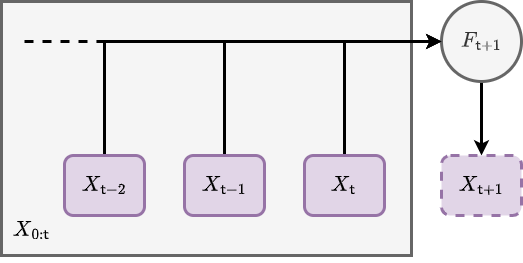
\includegraphics[width=10cm]{images/chapter-1-fundamental-loop.drawio.png}
\caption{Graph representation of Eq.~(\ref{eq:x-step-def}).}
\label{fig:fundamental-loop}
\end{figure}

The basic computational idea here is illustrated in Fig.~\ref{fig:fundamental-loop}; we iterate the matrix $X$ forward in time by a row, and use its previous version $X_{0:{\sf t}}$ as an entire matrix input into a function which populates the elements of its latest rows. In pseudocode you could easily write something with the same idea in it, and it would probably look something like the method diagram in Fig.~\ref{fig:fundamental-loop-code}.

\begin{figure}[h]
\centering
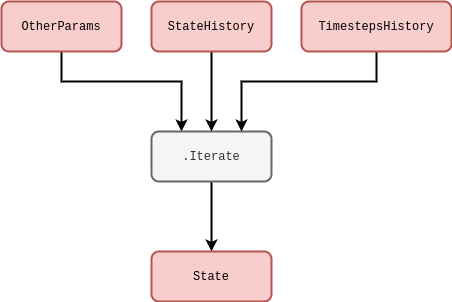
\includegraphics[width=10cm]{images/chapter-1-fundamental-loop-code.drawio.png}
\caption{Pseudocode representation of Eq.~(\ref{eq:x-step-def}).}
\label{fig:fundamental-loop-code}
\end{figure}

Pretty simple! But why go to all this trouble of storing matrix inputs for previous values of the same process? It's true that this is mostly redundant for \emph{Markovian} phenomena, i.e., processes where their only memory of their history is the most recent value they took. However, for a large class of stochastic processes a full memory\footnote{Or memory at least within some window.} of past values is essential to consistently construct the sample paths moving forward. This is true in particular for \emph{non-Markovian} phenomena, where the latest values don't just depend on the immediately previous ones but can depend on values which occured much earlier in the process as well.

For more complex physical models and integrators, the distinct notions of `numerical timestep' and `total elapsed continuous time' will crop up quite frequently. Hence, before moving on further details, it will be important to define the total elapsed time variable $t({\sf t})$ for processes which are defined in continuous time. Assuming that we have already defined some function $\delta t({\sf t})$ which returns the specific change in continuous time that corresponds to the step ${\sf t}-1 \rightarrow {\sf t}$, we will always be able to compute the total elapsed time through the relation
%%
\begin{align}
t({\sf t}) &= \sum^{{\sf t}}_{{\sf t}'=0}\delta t({\sf t}') \label{eq:t-steps-sum} \,.
\end{align}
%%
It's important to remember that our steps in continuous time may not be constant, so by defining the $\delta t({\sf t})$ function and summing over it we can enable this flexibility in the computation. In case the summation notation is no fun for programmers; we're simply adding up all of the differences in time to get a total.

So, now that we've mathematically defined a really general notion of iterating the stochastic process forward in time, it makes sense to discuss some simple examples. For instance, it is frequently possible to split $F$ up into deteministic (denoted $D$) and stochastic (denoted $S$) matrix-valued functions like so
%%
\begin{align}
& F^{i}_{{\sf t}+1}(X_{0:{\sf t}},z,{\sf t}) = D^{i}_{{\sf t}+1}(X_{0:{\sf t}},z,{\sf t}) + S^{i}_{{\sf t}+1}(X_{0:{\sf t}},z,{\sf t}) \,.
\end{align}
%%
In the case of stochastic processes with continuous sample paths, it's also nearly always the case with mathematical models of real-world systems that the deterministic part will at least contain the term $D^{i}_{{\sf t}+1}(X_{0:{\sf t}},z,{\sf t}) = X^i_{\sf t}$ because the overall system is described by some stochastic differential equation. This is not a really requirement in our general formalism, however.

What about the stochastic term? For example, if we wanted to consider a \emph{Wiener process noise}, we can define $W^i_{{\sf t}}$ is a sample from a Wiener process for each of the state dimensions indexed by $i$ and our formalism becomes
%%
\begin{align}
& S^{i}_{{\sf t}+1}(X_{0:{\sf t}},z,{\sf t}) = W^i_{{\sf t}+1}-W^i_{\sf t} \label{eq:wiener}\,.
\end{align}
%%
One draws the increments $W^i_{{\sf t}+1}-W^i_{\sf t}$ from a normal distribution with a mean of $0$ and a variance equal to the length of continuous time that the step corresponded to $\delta t({\sf t}+1)$, i.e., the probability density $P_{{\sf t}+1}(x^i)$ of the increments $x^i=W^i_{{\sf t}+1}-W^i_{\sf t}$ is
%%
\begin{align}
P_{{\sf t}+1}(x^i) &= {\sf NormalPDF}[x^i;0,\delta t({\sf t}+1)] \,.
\end{align}
%%
Note that for state spaces with dimensions $>1$, we could also allow for non-trivial cross-correlations between the noises in each dimension. In pseudocode, the Wiener process is schematically represented by Fig.~\ref{fig:wiener-process}.

\begin{figure}[h]
\centering
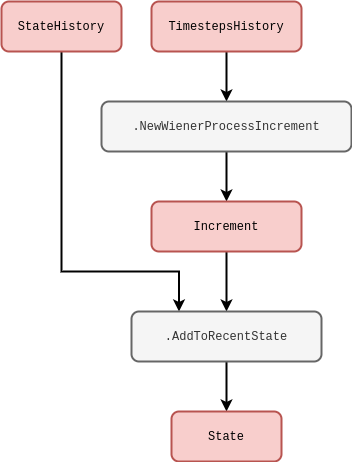
\includegraphics[width=8cm]{images/chapter-1-wiener-process.drawio.png}
\caption{Schematic of code for a Wiener process.}
\label{fig:wiener-process}
\end{figure}

In another example, to model \emph{geometric Brownian motion noise} we would simply have to multiply $X^i_{\sf t}$ to the Wiener process like so
%%
\begin{align}
& S^{i}_{{\sf t}+1}(X_{0:{\sf t}},z,{\sf t}) = X^i_{\sf t}(W^i_{{\sf t}+1}-W^i_{\sf t})\label{eq:gbm} \,.
\end{align}
%%
Here we have implicitly adopted the Itô interpretation to describe this stochastic integration. Given a carefully-defined integration scheme other interpretations of the noise would also be possible with our formalism too, e.g., Stratonovich\footnote{Which would implictly give $S^{i}_{{\sf t}+1}(X_{0:{\sf t}},z,{\sf t}) = (X^i_{{\sf t}+1}+X^i_{\sf t})(W^i_{{\sf t}+1}-W^i_{\sf t}) / 2$ for Eq.~(\ref{eq:gbm}).} or others within the more general `$\alpha$-family'~\cite{van1992stochastic,risken1996fokker,rog-will-2000}. The pseudocode for any of these should hoepfully be fairly straightforward to deduce based on the lines we've already written above.

\begin{figure}[h]
\centering
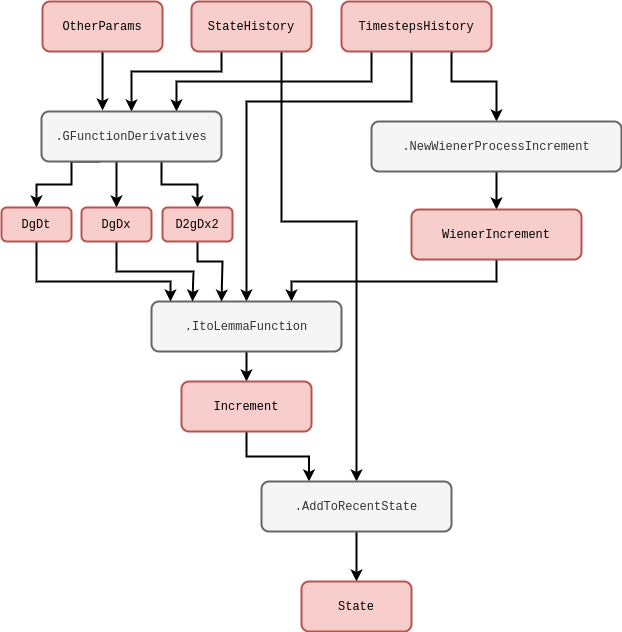
\includegraphics[width=12cm]{images/chapter-1-ito-lemma.drawio.png}
\caption{Schematic of code for Eq.~(\ref{eq:general-wiener}).}
\label{fig:ito-lemma}
\end{figure}

We can imagine even more general processes that are still Markovian. One example of these in a single-dimension state space would be to define the noise through some general function of the Wiener process like so
%%
\begin{align}
S^0_{{\sf t}+1}(X_{0:{\sf t}},z,{\sf t}) &= g[W^0_{{\sf t}+1},t({\sf t}+1)]-g[W^0_{\sf t}, t({\sf t})] \\
&= \bigg[ \frac{\partial g}{\partial t} + \frac{1}{2}\frac{\partial^2 g}{\partial x^2} \bigg] \delta t ({\sf t}+1) + \frac{\partial g}{\partial x} (W^0_{{\sf t}+1}-W^0_{\sf t}) \label{eq:general-wiener}\,,
\end{align}
%%
where $g(x,t)$ is some continuous function of its arguments which has been expanded out with Itô's Lemma on the second line. Note also that the computations in Eq.~(\ref{eq:general-wiener}) could be performed with numerical derivatives in principle, even if the function were extremely complicated. This is unlikely to be the best way to describe the process of interest, however, the mathematical expressions above can still be made a bit more meaningful to the programmer in this way. The pseudocode in general would look something like Fig.~\ref{fig:ito-lemma}.

Let's now look at a more complicated type of noise. For example, we might consider sampling from a \emph{fractional Brownian motion} process $[B_{H}]_{\sf t}$, where $H$ is known as the `Hurst exponent'. Following Ref.~\cite{decreusefond1999stochastic}, we can simulate this process in one of our state space dimensions by modifying the standard Wiener process by a fairly complicated integral factor which looks like this
%%
\begin{align}
S^{0}_{{\sf t}+1}(X_{0:{\sf t}},z,{\sf t}) &= \frac{(W^0_{{\sf t}+1} - W^0_{\sf t})}{\delta t({\sf t})}\int^{t({\sf t}+1)}_{t({\sf t})}{\rm d}t' \frac{(t'-t)^{H-\frac{1}{2}}}{\Gamma (H+\frac{1}{2})} {}_2F_1 \bigg( H-\frac{1}{2};\frac{1}{2}-H;H+\frac{1}{2};1-\frac{t'}{t}\bigg) \label{eq:fbm} \,,
\end{align}
%%
where $S^{0}_{{\sf t}+1}(X_{0:{\sf t}},z,{\sf t})=[B_{H}]_{{\sf t}+1}-[B_{H}]_{{\sf t}}$. The integral in Eq.~(\ref{eq:fbm}) can be approximated using an appropriate numerical procedure (like the trapezium rule, for instance). In the expression above, we have used the symbols ${}_2F_1$ and $\Gamma$ to denote the ordinary hypergeometric and gamma functions, respectively. A computational form of this integral is illustrated in Fig.~\ref{fig:fractional-brownian-motion} to try and disentangle some of the mathematics as a program.

\begin{figure}[h]
\centering
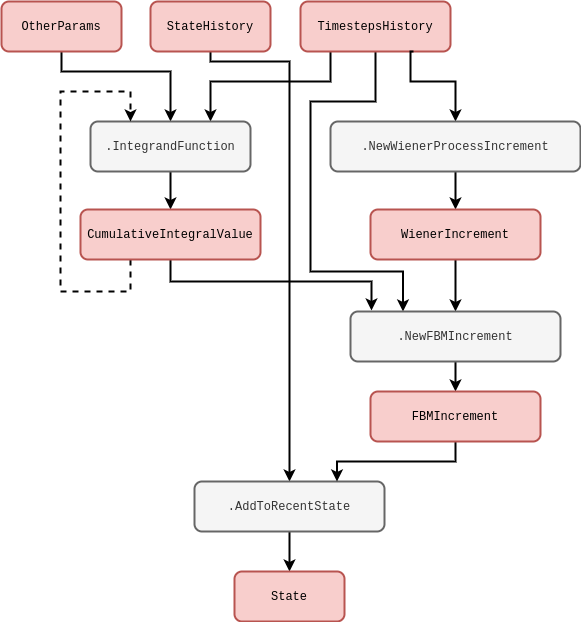
\includegraphics[width=11cm]{images/chapter-1-fractional-brownian-motion.drawio.png}
\caption{Schematic of code for Eq.~(\ref{eq:fbm}).}
\label{fig:fractional-brownian-motion}
\end{figure}

So far we have mostly been discussing noises with continuous sample paths, but we can easily adapt our computation to discontinuous sample paths as well. For instance, \emph{Poisson process noises} would generally take the form
%%
\begin{align}
S^{i}_{{\sf t}+1}(X_{0:{\sf t}},z,{\sf t}) &= [N_{\lambda}]^i_{{\sf t}+1}-[N_{\lambda}]^i_{\sf t}\,,
\end{align}
%%
where $[N_{\lambda}]^i_{\sf t}$ is a sample from a Poisson process with rate $\lambda$. One can think of this process as counting the number of events which have occured up to the given interval of time, where the intervals between each succesive event are exponentially distributed with mean $1/\lambda$. Such a simple counting process could be simulated exactly by explicitly setting a newly-drawn exponential variate to the next continuous time jump ${\delta t}({\sf t}+1)$ and iterating the counter. Other exact methods exist to handle more complicated processes involving more than one type of `event', such as the Gillespie algorithm~\cite{gillespie1977exact} --- though these techniques are not always be applicable in every situation.

Is using step size variation always possible? If we consider a \emph{time-inhomogeneous Poisson process noise}, which would generally take the form
%%
\begin{align}
S^{i}_{{\sf t}+1}(X_{0:{\sf t}},z,{\sf t}) &= [N_{\lambda ({\sf t}+1)}]^i_{{\sf t}+1}-[N_{\lambda ({\sf t})}]^i_{\sf t}\,,
\end{align}
%%
the rate $\lambda ({\sf t})$ has become a deterministically-varying function in time. In this instance, it likely not be accurate to simulate this process by drawing exponential intervals with a mean of $1/\lambda ({\sf t})$ because this mean could have changed by the end of the interval which was drawn. An alternative approach (which is more generally capable of simulating jump processes but is an approximation) first uses a small time interval $\tau$ such that the most likely thing to happen in this period is nothing, and then the probability of the event occuring is simply given by
%%
\begin{align}
p({\sf event}) &= \frac{\lambda ({\sf t})}{\lambda ({\sf t}) + \frac{1}{\tau}} \label{eq:rejection}\,.
\end{align}
%%
This idea can be applied to phenomena with an arbitrary number of events and works well as a generalised approach to event-based simulation, though its main limitation is worth remembering; in order to make the approximation good, $\tau$ often must be quite small and hence our simulator must churn through a lot of steps. From now on we'll refer to this well-known technique as the \emph{rejection method}. Fig.~\ref{fig:inhomogeneous-poisson} may also help to understand this concept from the programmer's perspective.

\begin{figure}[h]
\centering
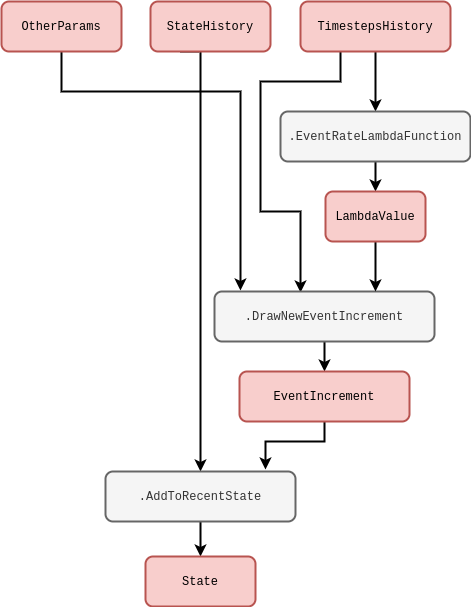
\includegraphics[width=9cm]{images/chapter-1-inhomogeneous-poisson.drawio.png}
\caption{Schematic of code for an inhomogeneous Poisson process.}
\label{fig:inhomogeneous-poisson}
\end{figure}

There are a few extensions to the simple Poisson process that introduce additional stochastic processes. \emph{Cox (doubly-stochastic) processes}, for instance, are basically where we replace the time-dependent rate $\lambda ({\sf t})$ with independent samples from some other stochastic process $\Lambda ({\sf t})$. For example, a Neyman-Scott process~\cite{neyman1958statistical} can be mapped as a special case of this because it uses a Poisson process on top of another Poisson process to create maps of spatially-distributed points. In our formalism, a two-state implementation of the Cox process noise would look like
%%
\begin{align}
S^{0}_{{\sf t}+1}(X_{0:{\sf t}},z,{\sf t}) &= \Lambda ({\sf t}+1) \\
S^{1}_{{\sf t}+1}(X_{0:{\sf t}},z,{\sf t}) &= [N_{S^{0}_{{\sf t}+1}}]^i_{{\sf t}+1}-[N_{S^{0}_{{\sf t}}}]^i_{\sf t}\,.
\end{align}
%%
This process could be simulated using the pseudocode we wrote for the time-inhomogeneous Poisson process previously --- where we would just replace \texttt{EventRateLambdaFunction} with a function that generates the stochastic rate $\Lambda ({\sf t})$.

Another extension is \emph{compound Poisson process noise}, where it's the count values $[N_{\lambda}]^i_{\sf t}$ which are replaced by independent samples $[J_{\lambda}]^i_{\sf t}$ from another probability distribution, i.e.,
%%
\begin{align}
S^{i}_{{\sf t}+1}(X_{0:{\sf t}},z,{\sf t}) &= [J_{\lambda}]^i_{{\sf t}+1}-[J_{\lambda}]^i_{\sf t}\,.
\end{align}
%%
Note that the rejection method of Eq.~(\ref{eq:rejection}) can be employed effectively to simulate any of these extensions as long as a sufficiently small $\tau$ is chosen. Once again, the pseudocode we wrote previously would be sufficient to simulate this process with one tweak: add into the \texttt{DrawNewEventIncrement} function the calling of a function which generates the $[J_{\lambda}]^i_{\sf t}$ samples and output these if the event occurs.

All of the examples we have discussed so far are Markovian. Given that we have explicitly constructed the formalism to handle non-Markovian phenomena as well, it would be worthwhile going some examples of this kind of process too. \emph{Self-exciting process noises} would generally take the form
%%
\begin{align}
S^{0}_{{\sf t}+1}(X_{0:{\sf t}},z,{\sf t}) &= {\cal I}_{{\sf t}+1} (X_{0:{\sf t}},z,{\sf t}) \\
S^{1}_{{\sf t}+1}(X_{0:{\sf t}},z,{\sf t}) &= [N_{S^{0}_{{\sf t}+1}}]^i_{{\sf t}+1}-[N_{S^{0}_{{\sf t}}}]^i_{\sf t} \,,
\end{align}
%%
where the stochastic rate ${\cal I}_{{\sf t}+1} (X_{0:{\sf t}},z,{\sf t})$ now depends on the history explicitly. Amongst other potential inputs we can see, e.g., Hawkes processes~\cite{hawkes1971spectra} as an example of above by substituting 
%%
\begin{align}
{\cal I}_{{\sf t}+1} (X_{0:{\sf t}},z,{\sf t}) &= \mu + \sum^{{\sf t}}_{{\sf t}'=0}\gamma [t({\sf t})-t({\sf t}')]S^{1}_{{\sf t}'} \,,
\end{align}
%%
where $\gamma$ is the `exciting kernel' and $\mu$ is some constant background rate. In order to simulate a Hawkes process using our formalism, the pseudocode would be something like Fig.~\ref{fig:hawkes-process}.

\begin{figure}[h]
\centering
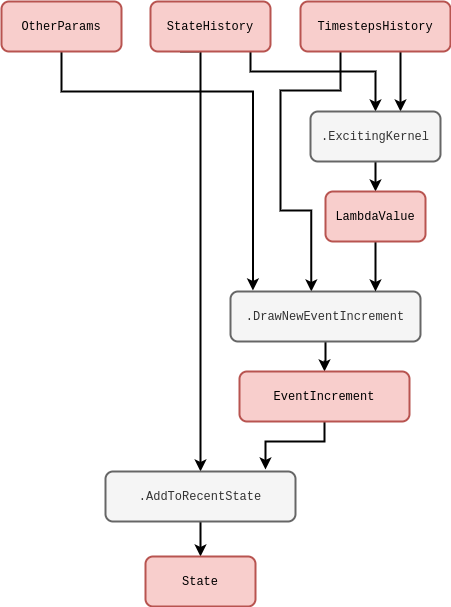
\includegraphics[width=9cm]{images/chapter-1-hawkes-process.drawio.png}
\caption{Schematic of code for a Hawkes process.}
\label{fig:hawkes-process}
\end{figure}

Note that this idea of integration kernels could also be applied back to our Wiener process. For example, another type of non-Markovian phenomenon that frequently arises across physical and life systems integrates the Wiener process history like so
%%
\begin{align}
S^{0}_{{\sf t}+1}(X_{0:{\sf t}},z,{\sf t}) &= W^0_{{\sf t}+1}-W^0_{\sf t}\\
S^{1}_{{\sf t}+1}(X_{0:{\sf t}},z,{\sf t}) &= u\sum^{{\sf t}}_{{\sf t}'=0}e^{-u[t({\sf t})-t({\sf t}')]} S^{0}_{{\sf t}'}\,,
\end{align}
%%
where $u$ is inversely proportional to the length of memory in continuous time.

\section{\sffamily Software design}

So we've proposed a computational formalism and then studied it in more detail to demonstrate that it can cope with a variety of different stochastic phenomena. Now we're ready to summarise what we want the stochadex software package to be able to do. But what's so complicated about Eq.~(\ref{eq:x-step-def})? Can't we just implement an iterative algorithm with a single function? It's true that the fundamental concept is very straightforward, but as we'll discuss in due course; the stochadex needs to have a lot of configurable features so that it's applicable in different situations. Ideally, the stochadex sampler should be designed to try and maintain a balance between performance and flexibility of utilisation.

If we begin with the obvious first set of criteria; we want to be able to freely configure the iteration function $F$ of Eq.~(\ref{eq:x-step-def}) and the timestep function $t$ of Eq.~(\ref{eq:t-steps-sum}) so that any process we want can be described. The point at which a simulation stops can also depend on some algorithm termination condition which the user should be able to specify up-front.

\begin{figure}[h]
\centering
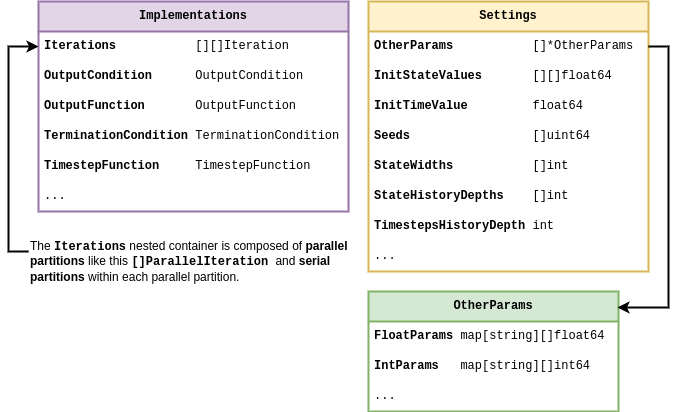
\includegraphics[width=13cm]{images/chapter-1-stochadex-data-types.drawio.png}
\caption{A relational summary of the configuration data types in the stochadex.}
\label{fig:data-types-design}
\end{figure}

Once the user has written the code to create these functions for the stochadex, we want to then be able to recall them in future only with configuration files while maintaining the possibility of changing their simulation run parameters. This flexibility should facilitate our uses for the simulation later in the book, and from this perspective it also makes sense that the parameters should include the random seed and initial state value.

The state history matrix $X$ should be configurable in terms of its number of rows --- what we'll call the `state width' --- and its number of columns --- what we'll call the `state history depth'. If we were to keep increasing the state width up to millions of elements or more, it's likely that on most machines the algorithm performance would grind to a halt when trying to iterate over the resulting $X$ within a single thread. Hence, before the algorithm or its performance in any more detail, we can pre-empt the requirement that $X$ should represented in computer memory by a set of partitioned matrices which are all capable of communicating to one-another downstream. In this paradigm, we'd like the user to be able to configure which state partitions are able to communicate with each other without having to write any new code.

For convenience, it seems sensible to also make the outputs from stochadex runs configurable. A user should be able to change the form of output that they want through, e.g., some specified function of $X$ at the time of outputting data. The times that the stochadex should output this data can also be decided by some user-specified condition so that the frequency of output is fully configurable as well. 

In summary, we've put together a schematic of configuration data types and their relationships in Fig.~\ref{fig:data-types-design}. In this diagram there is some indication of the data type that we propose to store each piece information in (in Go syntax), and the diagram as a whole should serve as a useful guide to the basic structure of configuration files for the stochadex.

It's clear that in order to simulate Eq.~(\ref{eq:x-step-def}), we need an interative algorithm which reapplies a user-specified function to the continually-updated history. But let's now return to the point we made earlier about how the performance of such an algorithm will depend on the size of the state history matrix $X$. The key bit of the algorithm design that isn't so straightforward is: how do we sucessfully split this state history up into separate partitions in memory while still enabling them to communicate effectively with each other? Other generalised simulation frameworks --- such as SimPy~\cite{simpy}, StoSpa~\cite{stospa} and FLAME GPU~\cite{flamegpu} --- have all approached this problem in different ways, and with different software architectures. 

In Fig.~\ref{fig:loop-design} we've illustrated what a loop involving separate state partitions looks like in the stochadex simulator. Each partition is handled by concurrently running execution threads of the same process, while a separate process may be used to handle the outputs from the algorithm. As the diagram shows, the main sequence of each loop iteration follows the pattern: 
%%
\begin{enumerate}
\item{The \texttt{PartitionCoordinator} requests more iterations from each state partition by sending an \texttt{IteratorInputMessage} to a concurrently running goroutine.}
\item{The \texttt{StateIterator} in each goroutine executes the iteration and stores the resulting state update in a variable.}
\item{Once all of the iterations have been completed, the \texttt{PartitionCoordinator} then requests each goroutine to update its relevant partition of the state history by sending another \texttt{IteratorInputMessage} to each.}
\end{enumerate}
%%
This pattern ensures that no partition has access to values in the state history which are out of sync with its current state in time, and hence prevents anachronisms from occuring in the overall state iteration. 

\begin{figure}[h]
\centering
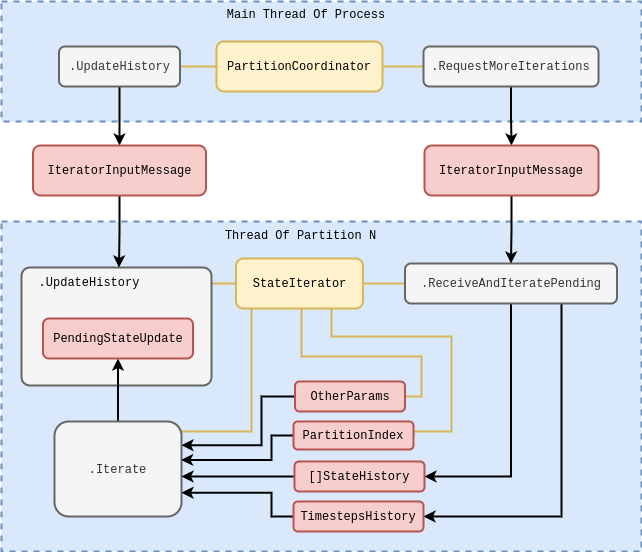
\includegraphics[width=13cm]{images/chapter-1-stochadex-loop.drawio.png}
\caption{Schematic for a step of the stochadex simulation algorithm.}
\label{fig:loop-design}
\end{figure}

It's also worth noting that while Fig.~\ref{fig:loop-design} illustrates only a single process; it's obviously true that we may run many of these whole diagrams at once to parallelise generating independent realisations of the simulation, if necessary.

As we stated at the beginning of this chapter: the full implementation of the stochadex can be found on GitHub by following this link: \href{https://github.com/umbralcalc/stochadex}{https://github.com/umbralcalc/stochadex}. Users can build the main binary executable of this repository and determine what configuration of the stochadex they would like to have through config at runtime (one can infer these configurations from Fig.~\ref{fig:data-types-design}). As Go is a statically typed language, this level of flexibility has been achieved using code templating proceeding runtime build and execution via \texttt{go run} `under-the-hood'. Users who find this particular execution pattern undesirable can also use all of the stochadex types, tools and methods as part of a standard library import.

In order to debug the simulation code and gain a more intuitive understanding of the outputs from a model as it is being developed, we have also written a lightweight frontend dashboard React~\cite{react} app in TypeScript to visualise any stochadex simulation as it is running. This dashboard can be launched by passing config at runtime to the main stochadex executable, and we have illustrated how all this fits together in a flowchart shown in Fig.~\ref{fig:stochadex-main}.

\begin{figure}[h]
\centering
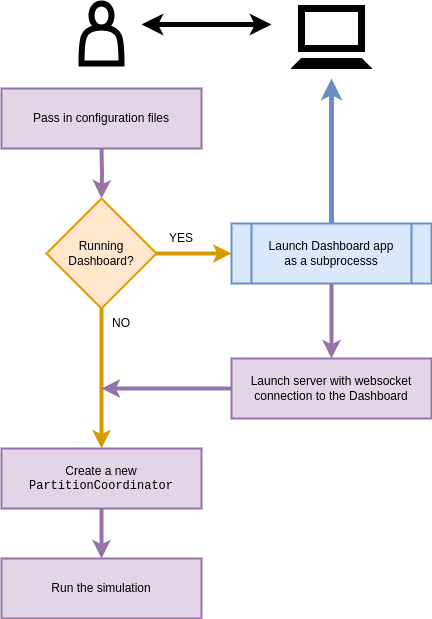
\includegraphics[width=9cm]{images/chapter-1-stochadex-main.drawio.png}
\caption{A diagram of the main stochadex binary executable.}
\label{fig:stochadex-main}
\end{figure}



\part*{
\includegraphics*[width=14cm]{images/page-design-2.png}}

\chapter{\sffamily Simulating a financial market}

{\bfseries\sffamily Concept.} The idea here is to use the Q-Hawkes processes and the Bouchaud work to come up with some interesting simulations of financial markets. 

\section{\sffamily Introducing Q-Hawkes processes}



\part*{
\includegraphics*[width=14cm]{images/page-design-3.png}}

\chapter{\sffamily Quantum jumps on generic networks}

{\bfseries\sffamily Concept.} The idea is to follow this sort of thing \href{https://en.wikipedia.org/wiki/Quantum_jump_method}{here} to simulate the Lindblad equation over an arbitrary network of entangled states.

\section{\sffamily The Lindblad equation}

\part*{{\sffamily Part 2. {\color{gray75} How do we then learn/identify the answer to Part 1 from real-world data?}}
\includegraphics*[width=14cm]{images/page-design-1.png}}

\chapter{\sffamily Empirical dynamical emulators}

{\bfseries\sffamily Concept.} To extend the formalism that we developed in previous chapters to enable the empirical emulation of real-world data in a probabilistic way. This technique should enable a researcher to model complex dynamical trends in the data very well; at the cost of making the abstract interpretation of the model less immediately comprehensible than the statistical inference models in some proceeding chapters. As our generalised framework applies to a wide variety stochastic phenomena, our emulator will be applicable to a great breadth of data modeling problems as well. We will also explore some examples which illustrate how our empirical emulator should be applied in practice and then follow this up with how the code is designed and implemented as part of a new software package called `learnadex'. For the mathematically-inclined, this chapter will take a detailed look at how our formalism can be extended to focus on probabilistic dynamical process emulation. For the programmers, the software described in this chapter lives in the public Git repository: \href{https://github.com/umbralcalc/learnadex}{https://github.com/umbralcalc/learnadex}.

\section{\sffamily Probabilistic formalism}

The key distinction between the methods that we will develop in this chapter and the ones in the proceeding chapters is in their utility when faced with the problem of attempting to model real-world data. In the proceeding chapter, we shall describe some powerful techniques that can be used most effectively when the researcher is aware of the family of models that generated the data. In the present chapter, we will go into the details of how a more `empirical' approach can be derived for dynamical process modeling in a probabilistic framework which locally adapts the model to the data through time. 

While we think that it's worth going into some mathematical detail to give a better sense of where our formalism comes from; we want to emphasise that the framework we discuss here is not especially new to the technical literature. We shall be using  well-known techniques, such as Gaussian processes~\cite{murphy2012machine}, and our overall framework is comparable to that of Empirical Dynamical Modeling (EDM)~\cite{sugihara1990nonlinear}, or perhaps some classic nonparametric local regression techniques such as LOWESS/Savitzky-Golay filtering~\cite{savitzky1964smoothing} as well. The novelties here, instead, lie more in the specifics of how we combine some of these ideas together when referencing the stochadex formalism, and how this manifests in designing more generally-applicable software for the user.

Before we are able to develop this empirical emulator, we need to return to the stochadex formalism that we introduced in the first chapter of this book. As we discussed at that point; this formalism is appropriate for sampling from nearly every stochastic phenomenon that one can think of. However, when trying robustly assess how far a model is from accurately describing a set of real-world data, trying to use only generated samples of the model process can be diffcult. Instead, in this section, we are going to extend this formalism to look at how probability theory can help with this data comparison problem in a systematic way.

So, how do we begin? In the first chapter, we defined the general stochastic process with the formula $X^{i}_{{\sf t}+1} = F^{i}_{{\sf t}+1}(X',z,{\sf t})$. This equation also has an implicit \emph{master equation} associated to it that fully describes the time evolution of the \emph{probability density function} $P_{{\sf t}+1}(x)$ of the most recent matrix row $x=X_{{\sf t}+1}$ at time ${\sf t}$. This can be written as
%%
\begin{align}
P_{{\sf t}+1}(x) &= \frac{1}{{\sf t}}\sum_{{\sf t}'=0}^{{\sf t}}\int_{\omega_{{\sf t}'}}{\rm d}x' P_{{\sf t}'}(x') P_{({\sf t}+1){\sf t}'}(x\vert x') \label{eq:master-x-cont} \,,
\end{align}
%%
where at the moment we are assuming the state space is continuous in each dimension and $P_{({\sf t}+1){\sf t}'}(x\vert x')$ is the conditional probability that the matrix row at time $({\sf t}+1)$ will be $x=X_{{\sf t}+1}$ given that the row at time ${\sf t}'$ was $x'=X_{{\sf t}'}$. This is a very general equation which should almost always apply to any continuous stochastic phenomenon we want to study in due course. To try and understand what this equation is saying we find it's helpful to think of an iterative relationship between probabilities; each of which is connected by their relative conditional probabilities. This kind of thinking is also illustrated in Fig.~\ref{fig:master-eqn}. Let's say we also wanted to program what this equation is saying as a function in Go. Using a Monte Carlo approximation for the integral domain, the code might look something like this.

\begin{lstlisting}[language=Go]
type StateVector  []float64

// returns a random draw of the possible state vectors at this timestep
func RandomPossibleStateVectors(timeStepNumber int) []StateVector {
    // return a slice of randomly-drawn possible state vectors 
    // corresponding to the integral domain at this timestep
}

// returns the conditional probability of the state vector at this timestep 
// given the value that the state vector had on a previous timestep
func StateVectorConditionalProbability(
    stateVector StateVector,
    timeStepNumber int,
    previousStateVector StateVector,
    previousTimeStepNumber int,
) float64 {
    // return the conditional probability value
}

// returns the probability of the state vector at this timestep
func StateVectorProbability(
    stateVector StateVector, 
    timeStepNumber int,
) float64 {
    prob := 0.0
    // loop over all the possible previous timesteps
    for t := 0; t < timeStepNumber; t++ {
        // loop over the randomly-drawn possible state vectors 
        // for this previous timestep
        possibleStateVectors := RandomPossibleStateVectors(t)
        for _, possibleStateVector := range possibleStateVectors {
            // note the recursion
            prob += StateVectorProbability(possibleStateVector, t)*
                StateVectorConditionalProbability(
                    stateVector,
                    timeStepNumber,
                    possibleStateVector, 
                    t,
                )
        }
        // normalisation for the Monte Carlo integration
        prob /= float64(len(possibleStateVectors))
    }
    // timestep normalisation
    prob /= float64(timeStepNumber)
    return prob
}
\end{lstlisting}

The factor of $1/{\sf t}$ in Eq.~(\ref{eq:master-x-cont}) is a normalisation factor --- this just normalises the sum of all probabilities to 1 given that there is a sum over ${\sf t}'$. Note that, if the process is defined over continuous time, we would need to replace 
%%
\begin{align}
\frac{1}{{\sf t}}\sum_{{\sf t}'=0}^{{\sf t}} \rightarrow \frac{1}{t({\sf t})}\sum_{{\sf t}'=0}^{{\sf t}}\delta t({\sf t}') \,.
\end{align}
%% 
But what is $\omega_{\sf t}$? You can think of this as just the domain of possible $x'$ inputs into the integral which will depend on the specific stochastic process we are looking at.

\begin{figure}[h]
\centering
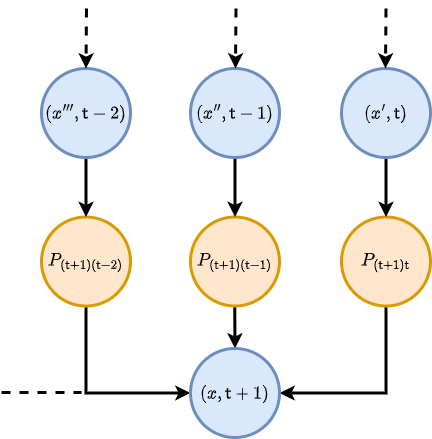
\includegraphics[width=8cm]{images/master-eq-graph.drawio.png}
\caption{Graph representation of Eq.~(\ref{eq:master-x-cont}).}
\label{fig:master-eqn}
\end{figure}

What if we wanted the joint distribution of both rows $P_{({\sf t}+1){\sf t}'}(x,x')$? One way to obtain this would be to extend Eq.~(\ref{eq:master-x-cont}) such that both matrix rows are marginalised over separately like so
%%
\begin{align}
&P_{({\sf t}+1){\sf t}'}(x,x') = \nonumber \\
&\qquad \frac{1}{({\sf t}'-1){\sf t}}\sum_{{\sf t}''=0}^{{\sf t}}\sum_{{\sf t}'''=0}^{{\sf t}'-1}\int_{\omega_{{\sf t}''}}{\rm d}x''\int_{\omega_{{\sf t}'''}}{\rm d}x''' P_{{\sf t}''{\sf t}'''}(x'', x''') P_{({\sf t}+1){\sf t}''}(x\vert x'')P_{{\sf t}'{\sf t}'''}(x'\vert x''') \label{eq:joint-master-x-cont} \,.
\end{align}
%%
Given Eqs.~(\ref{eq:master-x-cont}) and~(\ref{eq:joint-master-x-cont}) it's also possible to work out what the conditional probabilities would look like using the simple relation
%%
\begin{align}
P_{({\sf t}+1){\sf t}'}(x\vert x') &= \frac{P_{({\sf t}+1){\sf t}'}(x,x')}{P_{{\sf t}'}(x')} \label{eq:cond-master-x-cont} \,.
\end{align}
%%

The implicit notation in Eq.~(\ref{eq:master-x-cont}) can hide some staggering complexity. To analyse the system in more detail, we can also do a kind of Kramers-Moyal expansion~\cite{kramers1940brownian,moyal1949stochastic} for each point in time to approximate the overall equation like this
%%
\begin{align}
P_{{\sf t}+1}(x) &= \frac{1}{{\sf t}}\sum_{{\sf t}'=0}^{{\sf t}}P_{{\sf t}'}(x) - \frac{1}{{\sf t}}\sum_{{\sf t}'=0}^{{\sf t}}\sum_{i=1}^d\frac{\partial}{\partial x^i}\big[ \alpha^i_{({\sf t}+1){\sf t}'}(x)P_{{\sf t}'}(x)\big] \nonumber \\
& \qquad + \frac{1}{2{\sf t}}\sum_{{\sf t}'=0}^{{\sf t}}\sum_{i=1}^d\sum_{j=1}^d\frac{\partial}{\partial x^i}\frac{\partial}{\partial x^j}\big[ \beta^{ij}_{({\sf t}+1){\sf t}'}(x)P_{{\sf t}'}(x)\big] + \dots \label{eq:master-x-cont-kramers-moyal} \,,
\end{align}
%%
in which we have assumed that the state space is $d$-dimensional. In this expansion, we also needed to define these new integrals
%%
\begin{align}
\alpha^i_{({\sf t}+1){\sf t}'}(x) &=\int_{\omega_{{\sf t}'}} {\rm d}x'(x'-x)^iP_{({\sf t}+1){\sf t}'}(x'\vert x) \\
\beta^{ij}_{({\sf t}+1){\sf t}'}(x) &= \int_{\omega_{{\sf t}'}} {\rm d}x'(x'-x)^i(x'-x)^jP_{({\sf t}+1){\sf t}'}(x'\vert x) \,.
\end{align}
%%
So the matrix notation of Eq.~(\ref{eq:master-x-cont}) can indeed hide a very complicated calculation. Truncating the expansion at second-order, Eq.~(\ref{eq:master-x-cont-kramers-moyal}) tells us that there can be first and second derivatives contributing to the flow of probability to each element of the row $x=X_{{\sf t}+1}$ which depend on every element of the matrix $X'$. The probability does indeed \emph{flow}, in fact. We can define a quantity known as the `probability current' $J_{({\sf t}+1){\sf t}'}(x)$ from ${\sf t}'$ to $({\sf t}+1)$ which illustrates this through the following continuity relation
%%
\begin{align}
P_{{\sf t}+1}(x) - \frac{1}{{\sf t}}\sum_{{\sf t}'=0}^{{\sf t}}P_{{\sf t}'}(x) = \frac{1}{{\sf t}}\sum_{{\sf t}'=0}^{{\sf t}}\big[ P_{{\sf t}+1}(x) - P_{{\sf t}'}(x)\big] = - \frac{1}{{\sf t}}\sum_{{\sf t}'=0}^{{\sf t}}J_{({\sf t}+1){\sf t}'}(x) \,.
\end{align}
%%
By inspection of Eq.~(\ref{eq:master-x-cont-kramers-moyal}) we can therefore also deduce that
%%
\begin{align}
J^i_{({\sf t}+1){\sf t}'}(x) &= \alpha^i_{({\sf t}+1){\sf t}'}(x)P_{{\sf t}'}(x) - \frac{1}{2}\sum_{j=1}^d\frac{\partial}{\partial x^j}\big[ \beta^{ij}_{({\sf t}+1){\sf t}'}(x)P_{{\sf t}'}(x)\big] + \dots \,.
\end{align}
%%

What would happen if we assumed that $\alpha$ could be defined with just an arbitrary time-dependent function? In this instance, we mean
%%
\begin{align}
\alpha^i_{({\sf t}+1){\sf t}'}(x) &= f^i({\sf t}')-x^i \,,
\end{align}
%%
where $f({\sf t}')=f'$ is an arbitrary vector-valued function of the timestep. Using this function, we might then try to approximate $\beta^{ij}_{({\sf t}+1){\sf t}'}(x) \simeq \beta^{ij}_{({\sf t}+1){\sf t}'}(f') = 2K(\theta , {\sf t}' ; f')$ with the matrix $K$, which depends on both the timestep and a set of hyperparameters $\theta$. If we now also assume stationarity of $P_{{\sf t}'}(x)=P_{{\sf t}''}(x)$ for any ${\sf t}'$ and ${\sf t}''$ such that
%%
\begin{align}
P_{{\sf t}+1}(x) = \frac{1}{{\sf t}}\sum_{{\sf t}'=0}^{{\sf t}} P_{{\sf t}'}(x) \,,
\end{align}
%%
we can solve Eq.~(\ref{eq:master-x-cont-kramers-moyal}) to obtain the following stationary solution
%%
\begin{align}
P_{{\sf t}'}(x) &= {\sf MultivariateNormalPDF}[x;f',K(\theta , {\sf t}' ; f')]\label{eq:stat-sol-kramers-moyal}\,.
\end{align}
%%
Note in that last step the solution also required the identification that the flow of probability between timesteps vanishes uniquely for each and every ${\sf t}'$ such that $J_{({\sf t}+1){\sf t}'}(x)=0$. 

\begin{figure}[h]
\centering
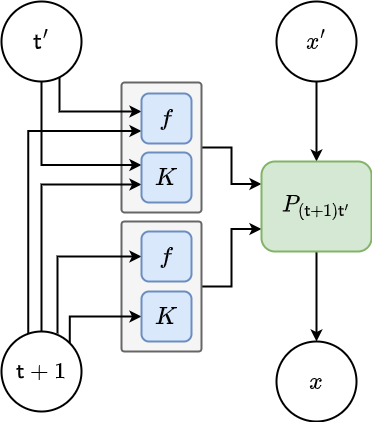
\includegraphics[width=8cm]{images/gp-like-diag.drawio.png}
\caption{Graph representation of the generative process implied by Eq.~(\ref{eq:stat-sol-kramers-moyal-cond}).}
\label{fig:stat-sol-kramers-moyal-cond}
\end{figure}

It's possible to take this derivation a bit further by expanding Eq.~(\ref{eq:joint-master-x-cont}) in a similar fashion, truncating it to second-order, assuming only time-dependent terms and then solving it in the stationary limit. By plugging this solution (and its corresponding marginal distribution equivalent) into Eq.~(\ref{eq:cond-master-x-cont}), you can get something that looks like this conditional distribution
%%
\begin{align}
P_{({\sf t}+1){\sf t}'}(x\vert x') &\propto {\rm exp}\bigg\{ -\frac{1}{2}\sum^d_{i=1}\sum^d_{j=1}(x-f)^i \big[K^{-1}(\theta , {\sf t}+1,{\sf t}+1; f,f)\big]^{ij}(x-f)^j \nonumber \\
& \qquad \qquad + \sum^d_{i=1}\sum^d_{j=1}(x-f)^i \big[ K^{-1}(\theta , {\sf t}+1,{\sf t}'; f,f')\big]^{ij}(x'-f')^j  \bigg\} \label{eq:stat-sol-kramers-moyal-cond}\,,
\end{align}
%%
where $f({\sf t}+1)=f$ and $K(\theta , {\sf t}+1,{\sf t}'; f,f')$ is some arbitrary covariance matrix that encodes how the correlation structure varies with the between compared states at two different timesteps and $K^{-1}$ denotes taking its inverse. Note also that the inequality $({\sf t}+1)>{\sf t}'$ must always hold.

Eq.~(\ref{eq:stat-sol-kramers-moyal-cond}) may look a bit familiar to some readers who like using Gaussian processes from the machine learning literature~\cite{murphy2012machine} --- this version implies a \emph{generative} model for a future $x$ value (which we've illustrated in Fig~\ref{fig:stat-sol-kramers-moyal-cond}), in contrast to the more standard equation used to \emph{infer} values of $f$. These are two sides of the same coin though. 

Written in Go, the conditional probability in Eq.~(\ref{eq:stat-sol-kramers-moyal-cond}) could be computed by performing the summations over each element of the state vectors. We've given a rough idea of what this code would look like below.

\begin{lstlisting}[language=Go]
import "math"

type KernelParams []float64

// returns the f function value for a given timestep
func F(timestepNumber int) []float64 {
    // return value
}

// returns the inverse-K matrix for the input timesteps and 
// params (theta in the text)
func inverseK(
    params KernelParams,
    timestepNumber int, 
    previousTimeStepNumber int,
) [][]float64 {
    // return value
}

// returns the conditional probability of the state vector at this timestep 
// given the value that the state vector had on a previous timestep
func StateVectorConditionalProbability(
    stateVector StateVector,
    timeStepNumber int,
    previousStateVector StateVector,
    previousTimeStepNumber int,
) float64 {
    // set the params from somewhere
    var kernelParams KernelParams
    
    // get the f-function values for both timesteps
    f := F(timeStepNumber)
    previousF := F(previousTimeStepNumber)
    
    // get the inverse-K matrices for the latest timestep
    // and also when both timesteps are input
    invK := inverseK(kernelParams, timeStepNumber, timeStepNumber)
    bothInvK := inverseK(
        kernelParams, 
        timeStepNumber, 
        previousTimeStepNumber,
    )

    // loop over terms to add to the log-probability
    logProbability := 0.0
    for i := range stateVector {
        for j := range stateVector {
            logProbability += -(stateVector[i] - f[i])*
                invK[i][j]*(stateVector[j] - f[j])/2.0
            logProbability += (stateVector[i] - f[i])*
                bothInvK[i][j]*(previousStateVector[j] - previousF[j])
        }
    }
    return math.Exp(logProbability)
}
\end{lstlisting}

In Eq.~(\ref{eq:stat-sol-kramers-moyal-cond}) we are implicitly approximating $\beta^{ij}_{({\sf t}+1){\sf t}'}(x,x') \simeq \beta^{ij}_{({\sf t}+1){\sf t}'}(f,f')$, which can also be thought of as a zeroth-order `mean-field' expansion (here just a Taylor series in $x$ and $x'$) of the covariance matrix. If we were to continue this approximation up to second order, we would obtain 
%%
\begin{align}
& K(\theta , {\sf t}+1, {\sf t}'; x,x') \simeq \nonumber \\
& K + \sum_{i=1}^d(x-f)^i\frac{\partial K}{(\partial x)^i} + \sum_{i=1}^d(x'-f')^i\frac{\partial K}{(\partial x')^i} + \frac{1}{2}\sum_{i=1}^d\sum_{j=1}^d (x-f)^i\frac{\partial^2 K}{(\partial x)^i(\partial x)^j}(x-f)^j \nonumber \\
&+ \frac{1}{2}\sum_{i=1}^d\sum_{j=1}^d (x'-f')^i\frac{\partial^2 K}{(\partial x')^i(\partial x')^j}(x'-f')^j + \sum_{i=1}^d\sum_{j=1}^d (x-f)^i\frac{\partial^2 K}{(\partial x)^i(\partial x')^j}(x'-f')^j \label{eq:dali-covariance}\,.
\end{align}
%%
where all of the references to `$K$' above are evaluated using $x=f$ and $x'=f'$ after any derivatives of the variable have been taken. This kind of derivative approximation of $K$ is known in other contexts as the DALI method~\cite{sellentin2014breaking, dali}. In our case, this derivative approximation manifests as an expansion of $K$ to include terms which extend the powers of $x$ and $x'$ all the way up to fourth-order when applied to Eq.~(\ref{eq:stat-sol-kramers-moyal-cond}). The benefit of this expansion in Eq.~(\ref{eq:stat-sol-kramers-moyal-cond}) as opposed to approximating the probability distribution through Gram-Charlier A series or Edgeworth series~\cite{kolassa2006series}, is that in the latter cases it is much more difficult to ensure that the probability distribution is properly normalised.

By extending the procedure which obtains the joint distribution update in Eq.~(\ref{eq:joint-master-x-cont}) and uses Eq.~(\ref{eq:cond-master-x-cont}) to higher and higher orders of joint distribution $P_{({\sf t}+1){\sf t}'{\sf t}''}(x, x', x'')$, $P_{({\sf t}+1){\sf t}'{\sf t}''{\sf t}'''}(x, x', x'', x''')$, etc. you can derive equations for conditional distributions like $P_{({\sf t}+1){\sf t}'{\sf t}''}(x; x', x'')$ which are able to describe higher-order correlations between state vectors. If we apply the DALI expansion of $K$ to include higher-order dependencies on $x''$ and $x'''$, we obtain this monster expression
%%
\begin{align}
& K(\theta , {\sf t}+1, {\sf t}', {\sf t}'', {\sf t}'''; x,x',x'',x''') \simeq \nonumber \\
& K + \sum_{i=1}^d(x-f)^i\frac{\partial K}{(\partial x)^i} + \sum_{i=1}^d(x'-f')^i\frac{\partial K}{(\partial x')^i} + \sum_{i=1}^d(x''-f'')^i\frac{\partial K}{(\partial x'')^i} + \sum_{i=1}^d(x'''-f''')^i\frac{\partial K}{(\partial x''')^i} \nonumber \\
& + \frac{1}{2}\sum_{i=1}^d\sum_{j=1}^d (x-f)^i\frac{\partial^2 K}{(\partial x)^i(\partial x)^j}(x-f)^j + \frac{1}{2}\sum_{i=1}^d\sum_{j=1}^d (x'-f')^i\frac{\partial^2 K}{(\partial x')^i(\partial x')^j}(x'-f')^j \nonumber \\
&+ \frac{1}{2}\sum_{i=1}^d\sum_{j=1}^d (x''-f'')^i\frac{\partial^2 K}{(\partial x'')^i(\partial x'')^j}(x''-f'')^j + \frac{1}{2}\sum_{i=1}^d\sum_{j=1}^d (x'''-f''')^i\frac{\partial^2 K}{(\partial x''')^i(\partial x''')^j}(x'''-f''')^j \nonumber \\
&+ \sum_{i=1}^d\sum_{j=1}^d (x-f)^i\frac{\partial^2 K}{(\partial x)^i(\partial x')^j}(x'-f')^j + \sum_{i=1}^d\sum_{j=1}^d (x-f)^i\frac{\partial^2 K}{(\partial x)^i(\partial x'')^j}(x''-f'')^j \nonumber \\
&+ \sum_{i=1}^d\sum_{j=1}^d (x-f)^i\frac{\partial^2 K}{(\partial x)^i(\partial x''')^j}(x'''-f''')^j + \sum_{i=1}^d\sum_{j=1}^d (x'-f')^i\frac{\partial^2 K}{(\partial x')^i(\partial x'')^j}(x''-f'')^j \nonumber \\
&+ \sum_{i=1}^d\sum_{j=1}^d (x'-f')^i\frac{\partial^2 K}{(\partial x')^i(\partial x''')^j}(x'''-f''')^j + \sum_{i=1}^d\sum_{j=1}^d (x''-f'')^i\frac{\partial^2 K}{(\partial x'')^i(\partial x''')^j}(x'''-f''')^j \label{eq:dali-covariance-higher}\,,
\end{align}
%%
where, once again, all of the references to `$K$' above are evaluated using $x=f$, $x'=f'$, $x''=f''$ and $x'''=f'''$ after any derivatives of the variable have been taken. Note also in the expression above, we have extended the shorthand notation to include $f({\sf t}'')=f''$ and $f({\sf t}''')=f'''$, where these new timesteps must also fit into the general inequality $({\sf t}+1)>{\sf t}'>{\sf t}''>{\sf t}'''$.

We've already mentioned that the derivative expansion (or DALI method) used in Eqs.~(\ref{eq:dali-covariance}) and~(\ref{eq:dali-covariance-higher}) is in a different context to where it was employed in Refs.~\cite{sellentin2014breaking, dali}. In our case, the probability distribution that we are trying to approximate contains out-of-time-order correlations in a similar fashion to those studied in quantum mechanics~\cite{hashimoto2017out,García-Mata:2023} (though we are obviously only talking about a classical statistical analogue in this case). Hence, if $K$ is a matrix which encodes second-order (pairwise) out-of-time order correlations, the derivatives of this matrix in Eq.~(\ref{eq:dali-covariance}) are higher-rank\footnote{By `higher-rank' here we specifically mean objects which have more indices than just a matrix $M^{ij}\rightarrow M^{ijk\dots}$.} objects which encode higher-order correlations between state vectors at different time points. Despite these expressions appearing as more complex than the second-order version, the methodology for using them in a generative model like Eq.~(\ref{eq:stat-sol-kramers-moyal-cond}), or for leveraging them to infer the $f({\sf t})$ function (as is done in Gaussian process inference) can be much the same. We'll get into all how this could be done in the next section. 

What other processes can be described by Eq.~(\ref{eq:master-x-cont})? For Markovian phenomena, the equation no longer depends on timesteps older than the immediately previous one, hence the expression reduces to just
%%
\begin{align}
P_{{\sf t}+1}(x) &= \int_{\omega_{\sf t}}{\rm d}x' P_{\sf t}(x') P_{({\sf t}+1){\sf t}}(x\vert x') \label{eq:master-x-cont-markov} \,.
\end{align}
%%
It's also easy to show that Eq.~(\ref{eq:master-x-cont-kramers-moyal}) naturally simplifies into the more usually applied Kramers-Moyal expansion when considering a Markovian process --- you just remove the sum over ${\sf t}'$ and the $1/{\sf t}$ normalisation factor. 

Note that an analog of Eq.~(\ref{eq:master-x-cont}) exists for discrete state spaces as well. We just need to replace the integral with a sum and the schematic would look something like this
%%
\begin{align}
P_{{\sf t}+1}(x) &= \frac{1}{{\sf t}}\sum_{{\sf t}'=0}^{\sf t}\sum_{\omega_{{\sf t}'}} P_{{\sf t}'}(x') P_{({\sf t}+1){\sf t}'}(x \vert x') \label{eq:master-x-disc} \,,
\end{align}
%%
where we note that the $P$'s in the expression above all now refer to \emph{probability mass functions}. Because the state space is now discrete, we cannot immediately intuit an approximative expansion from this expression. 

As a brief mathematical aside; if you're really determined to use a similar approach to the one we derived above, you can rewrite it in terms of continuous-valued characteristic functions like this
%%
\begin{align}
\varphi_{{\sf t}+1}(s) &= \frac{1}{{\sf t}}\sum_{{\sf t}'=0}^{\sf t}\int_{\ell_{{\sf t}'}}{\rm d}s' {\cal C}(s') \varphi_{{\sf t}'}(s') \varphi_{({\sf t}+1){\sf t}'}(s \vert s') \label{eq:master-x-disc-char} \\
{\cal C}(s') &= \frac{1}{(2\pi )^d}\sum_{\omega_{{\sf t}'}}e^{-i(s'\cdot x')} \,,
\end{align}
%%
where $\ell_{{\sf t}'}$ defines all the continuous values that the vector $s'$ can possibly have at time ${\sf t}'$. In the expression above, ${\cal C}(s')$ acts like is a kind of comb\footnote{This is very similar to how a `Dirac comb' works in signal processing~\cite{brandwood2012fourier}.} to map the continuous frequency domain of $s'$ onto the discrete state space of $x'$. Note also that ${\cal C}(s')$ uses the imaginary number $i$ and, to be visually tidier, the dot product notation $a\cdot b$ just means the sum of vector elements: $a\cdot b = \sum_{\forall k}a^kb^k$. In principle, one can perform an approximative expansion on Eq.~(\ref{eq:master-x-disc-char}) like we did for continuous state spaces. This isn't always the most practical way of analysing the system though. 

We have one more important example to discuss and then we can cap off this more mathematical section. In the even-simpler case where $x$ is just a vector of binary `on' or `off' states, Eq.~(\ref{eq:master-x-disc}) reduces to
%%
\begin{align}
P^i_{{\sf t}+1} &= \frac{1}{{\sf t}}\sum_{{\sf t}'=0}^{\sf t} \sum_{j=1}^d P^j_{{\sf t}'} P^{ij}_{({\sf t}+1){\sf t}'} = \frac{1}{{\sf t}}\sum_{{\sf t}'=0}^{\sf t} \sum_{j=1}^d \big[ P^j_{{\sf t}'} A^{ij}_{({\sf t}+1){\sf t}'} + (1-P^j_{{\sf t}'}) B^{ij}_{({\sf t}+1){\sf t}'} \big] \label{eq:master-x-disc-binary}\,,
\end{align}
%% 
where $P^i_{{\sf t}'}$ now represents the probability that element $x^i=1$ (is `on') at time ${\sf t}'$. The matrices $A$ and $B$ are defined as conditional probabilities where the previous state in time $P^j_{{\sf t}'}$ was either `on' or `off', respectively.

In this section, we looked into how the mathematical formalism used in the stochadex could be extended with probability theory. Now that we have more of a sense of how this formalism works, we are ready to move on to designing the algorithms for our emulator. So let's go!

\section{\sffamily Emulator algorithms}

Plan of action for this section.
\begin{itemize}
\item{Algorithm where the emulator is learned first as a Gaussian process and then correction coefficients at higher orders are learned afterwards with parametric kernels defined over the correction to the covariance kernel.}
\item{In order to stabilise the algorithm to sample size fluctuations, a stochastic gradient descent method to optimize would work well with ${\rm E}[\ln P_{({\sf t}+1){\sf t}',{\sf t}'',{\sf t}'''}(x\vert x', x'', x''')]$ so the expectation values like ${\rm E}[(x-f)(x'-f')(x''-f'')]$ end up being used directly in the optimisation anyway!}
\item{Investigate how the learned kernel shapes end up looking compared to the binned raw data.}
\end{itemize}

The parametric algorithm simply needs the $K$-functions to be specified and then an optimiser can run over the data values to simultaneously attempt to obtain $\theta$ and $f$ values. 

Helpful to write the basic structure of algorithm out in Go.

\section{\sffamily Software design}



\part*{
\includegraphics*[width=14cm]{images/page-design-1.png}}

\chapter{\sffamily Inferring dynamical 2D maps}

{\bfseries\sffamily Concept.} The idea here is 


\section{\sffamily Adapting the stochadex formalism}

\part*{
\includegraphics*[width=14cm]{images/page-design-1.png}}

\chapter{\sffamily Learning from ants on curved surfaces}

{\bfseries\sffamily Concept.} The idea here is 

\section{\sffamily Diffusive limits for ant interactions}

\part*{
\includegraphics*[width=14cm]{images/page-design-1.png}}

\chapter{\sffamily A world of hydrodynamic ensembles}

{\bfseries\sffamily Concept.} The idea here is 


\section{\sffamily The Boltzmann/Navier-Stokes equations}

\part*{
\includegraphics*[width=14cm]{images/page-design-1.png}}

\chapter{\sffamily Generalised statistical inference tools}

{\bfseries\sffamily Concept.} The idea here is to extend the stochadex with tools for very generalised statistical inference of an explicit model (Bayesian and Frequentist - both with likelihood likelihood-free ABC algorithms and the like) that will work in nearly every situation where the user knows the model space. Probably need to exploit the phase space analogy of the formalism.

\section{\sffamily Likelihood-free methods}

\part*{{\sffamily Part 3. {\color{gray75} How do we simulate a general set of control policies to interact with the answer to Part 1?}}
\includegraphics*[width=14cm]{images/page-design-1.png}}

\chapter{\sffamily Interacting with systems in general}

{\bfseries\sffamily Concept.} To design and build a software which can interact with stochastic processes of any kind, either manually through user input, or automatically by introducing a `policy'. The mathematical formalism and software that we introduce here will serve as a common language and interface for any simulation studies into manipulating real world phenomena, and will enable the learning of control algorithms in later chapters of this book. We will implement this new interaction software as an extension to the stochadex package. For the mathematically-inclined, this chapter will cover how interactions are structured in theory by adding some new concepts to the stochadex formalism and illustrating with some simple examples. For the programmers, the public Git repository for the code described in this chapter can be found here: \href{https://github.com/umbralcalc/stochadex}{https://github.com/umbralcalc/stochadex}.

\section{\sffamily Formalising general interactions}

Let's start by considering how we might adapt the mathematical formalism we have been using so far to be able to take actions which can manipulate the state at each timestep. Using the mathematical notation that we inherited from the stochadex, we may extend the formula for updating the state history matrix $X_{0:{\sf t}}\rightarrow X_{0:{\sf t}+1}$ to include a new layer of possible interactions which is facilitated by a new vector-valued `take action' function $G_{{\sf t}}$. In doing so we shall be defining the domain of an acting entity in the stochastic process environment --- which we shall hereafter refer to as simply the `agent'.

During a timestep over which actions are performed by the agent, the stochadex state update formula can be extended to include interactions by composition with the original state update function like so
%%
\begin{align}
X_{{\sf t}+1}^i &= G^i_{{\sf t}+1}[F_{{\sf t}+1}(X_{0:{\sf t}}, z, {\sf t}), A_{{\sf t}+1}] = {\cal F}^i_{{\sf t}+1}(X_{0:{\sf t}}, z, A_{{\sf t}+1}, {\sf t}) \label{eq:generalised-state-actions} \,,
\end{align}
%%
where we have also introduced the concept of the `actions' performed $A_{{\sf t}+1}$ on the system; some vector of parameters which define what actions are taken at timestep ${\sf t}+1$. The code for the new iteration formula would look something like Fig.~\ref{fig:iterations-with-actions}.

\begin{figure}[h]
\centering
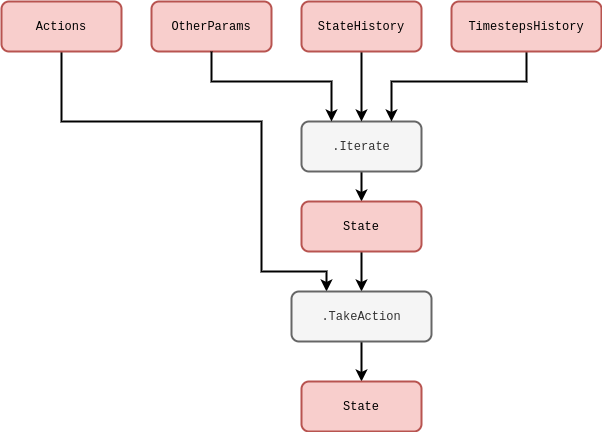
\includegraphics[width=11cm]{images/chapter-9-iterations-with-actions.drawio.png}
\caption{Code schematic of Eq.~(\ref{eq:generalised-state-actions}).}
\label{fig:iterations-with-actions}
\end{figure}

So far, Eq.~(\ref{eq:generalised-state-actions}) on its own will allow the agent to take actions that are scheduled up front through some fixed process or perhaps through user interaction via a game interface. So what's next? In order to start creating algorithms which will act on the system state for us, we need to develop a formalism which `closes the loop' by feeding information back from the stochastic process to the agent's decision-making algorithm.

If we use $A_{0:{\sf t}+1}$ a referring to the matrix of historically-taken actions which up to time ${\sf t}+1$, we can build up a more generalised, non-Markovian picture of automated interactions with the system which matches the notation we are already using for $X_{0:{\sf t}+1}$. Let us now define a Non-Markovian Decision Process (NMDP) as a probabilistic model which draws an actions matrix $A_{0:{\sf t}+1}=A$ from a `policy' distribution $\Pi_{({\sf t}+1){\sf t}}(A\vert X,\theta)$ given $X_{0:{\sf t}}=X$ and a new vector of parameters which fully specify the automated interations. Using the probabilistic notation from the previous part of the book, the joint probability that $X_{0:{\sf t}+1}=X$ and $A_{0:{\sf t}+1}=A$ at time ${\sf t}+1$ is
%%
\begin{align}
P_{{\sf t}+1}(X,A\vert z, \theta ) &= P_{{\sf t}}(X'\vert z,\theta ) \, \Pi_{({\sf t}+1){\sf t}}(A\vert X',\theta)P_{({\sf t}+1){\sf t}}(x\vert X',z,A) \label{eq:joint-prob-x-and-a} \,,
\end{align}
%%
where we recall that $P_{({\sf t}+1){\sf t}}(x\vert X',z,A)$ is the conditional probability of $X_{{\sf t}+1}=x$ given $X_{0:{\sf t}}=
X'$ and $z$ that we have encountered before, but it now requires $A_{0:{\sf t}+1}=A$ as another given input. We have illustrated Eq.~(\ref{eq:generalised-state-actions}) and how it relates to the policy distribution of Eq.~(\ref{eq:joint-prob-x-and-a}) with a new graph representation in Fig.~\ref{fig:fundamental-loop-with-actions}.

\begin{figure}[h]
\centering
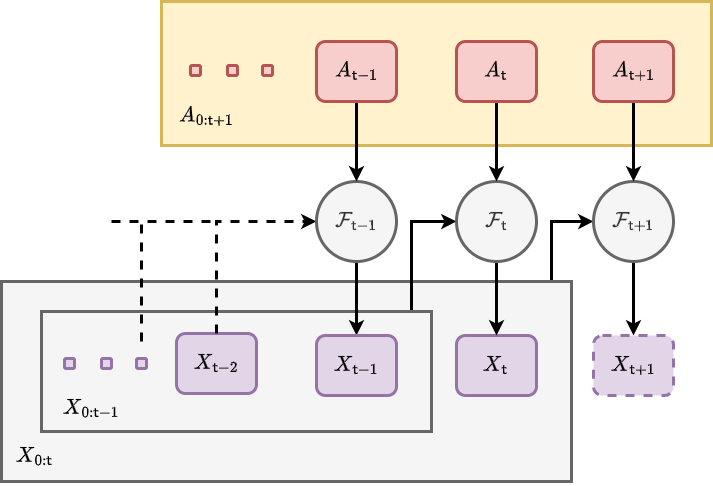
\includegraphics[width=11cm]{images/chapter-9-fundamental-loop-with-actions.drawio.png}
\caption{Graph representation of Eq.~(\ref{eq:generalised-state-actions}) with the policy distribution of Eq.~(\ref{eq:joint-prob-x-and-a}).}
\label{fig:fundamental-loop-with-actions}
\end{figure}

For additional clarity, let's take a moment to think about what $\Pi_{({\sf t}+1){\sf t}}(A\vert X,\theta)$ represents and how generally descriptive it can be. If an agent is acting under and entirely deterministic policy, then the policy distribution may be simplified to a direct function mapping which is parameterised by $\theta$. At the other extreme, the distribution may also describe a fully stochastic policy where actions are drawn randomly in time. If we combine this consideration of noise with the observation that policies described by a distribution $\Pi_{({\sf t}+1){\sf t}}(A\vert X,\theta)$ permit a memory of past actions and states, it's easy to see that this structure can be used in a wide variety of different use cases.

By marginalising over Eq.~(\ref{eq:joint-prob-x-and-a}) we find an updated probabilistic iteration formula for the stochastic process state which now takes the influence of agent actions into account
%%
\begin{align}
P_{{\sf t}+1}(X\vert z,\theta ) &= \int_{\Xi_{{\sf t}+1}}{\rm d}A \, P_{{\sf t}}(X'\vert z,\theta ) \, \Pi_{({\sf t}+1){\sf t}}(A\vert X',\theta)P_{({\sf t}+1){\sf t}}(x\vert X',z,A)  \,.
\end{align}
%%
This relationship will be very useful in the last part of this book when we begin to look at optimising control algorithms.

\textcolor{red}{
Think up some simple example categories of control and go through them here:
\begin{itemize}
\item{Markovian and non-Markovian decision processes}
\item{Discrete action decision processes (like bandit problem) --- choosing between website layouts for E-commerce~\cite{liu2021map}, sensor measurement scheduling, sequential design of large-scale scientific experiments }
\item{Continuously-acting decision processes --- controlling the temperature of chemical reactions (such as those in a brewery), spacecraft control~\cite{tipaldi2022reinforcement} and guidance systems, autonomous vehicles }
\item{Continuous event-based acting decision processes --- manager of a sports team, controlling traffic, managing disease spread, financial market portfolio optimisation }
\end{itemize}
}

\part*{
\includegraphics*[width=14cm]{images/page-design-1.png}}

\chapter{\sffamily Angling for freshwater fish}

{\bfseries\sffamily Concept.} The idea here is 

\section{\sffamily A large-scale Lotka-Volterra model}

Inspired by the empirical dynamical modeling approach to sockeye salmon in Ref.~\cite{ye2015equation}, but also desiring a generative model which has some link to the classic causal models promoted by mathematical ecology; the goal here is to create and calibrate a stochastic model which predicts the fish counts, weights, lengths and ages for each species in each area based on the past system states. To do this, we will combine some well-known models from mathematical ecology with supervised learning.

The one-step master equation for the proposed stochastic simulation is given implictly by

\begin{align}
\frac{{\rm d}}{{\rm d} t} P(\dots, n_{i}, \dots, t) &= \sum_{\forall i}{\cal T}^{+}_{i}(\dots, n_i-1, \dots, {\sf f}, t)P(\dots, n_{i}-1, \dots, t) \\
&+ \sum_{\forall i}{\cal T}^{-}_{i}(\dots, n_i+1, \dots, {\sf f}, t)P(\dots, n_{i}+1, \dots, t) \\
&- \sum_{\forall i}\bigg[ {\cal T}^{+}_{i}(\dots, n_i, \dots, {\sf f}, t) + {\cal T}^{-}_{i}(\dots, n_i, \dots, {\sf f}, t) \bigg] P(\dots, n_{i}, \dots,t) \,,
\end{align}

where the time $t$ is defined in units of years and ${\cal T}^{+}_{i}$ and ${\cal T}^{-}_{i}$ are the transition coefficients for the $i$-th species, which depend not only on the counts for all species $n_1, n_2, \dots$, but also (in principle) on a larger feature space ${\sf f}$ generated by the available data up to time $t$.

The famous Lotka-Volterra system, with some modficiations for fishing and a larger set of species, would suggest transition coefficients of the form


\begin{align}
{\cal T}^{+}_{i}(\dots, n_i, \dots, {\sf f}, t) = {\cal T}^{+}_{i}(\dots, n_i, \dots) &= \Lambda_{i}(n_{i}) + n_{i}\alpha_{i}\sum_{\forall i' \, {\sf prey}}n_{i'}\\
{\cal T}^{-}_{i}(\dots, n_i, \dots, {\sf f}, t) = {\cal T}^{-}_{i}(\dots, n_i, \dots) &= n_{i}\mu_{i} +  n_{i}\gamma_{i} + n_{i}\beta_{i} \sum_{\forall i' \, {\sf pred}} n_{i'} \,,
\end{align}


where: $\Lambda_{i}(n_{i}) = \tilde{\Lambda_{i}}n_{i}e^{-\lambda_i(n_{i}-1)}$ is the density-dependent birth rate; $\mu_{i}$ is the species death rate; $\alpha_{i}$ is the increase in the baseline birth rate per fish caused by the increase in prey population; $\beta_{i}$ is the rate per fish of predation of the species; and $\gamma_{i}$ accounts for the rate of recreational fishing per fish of the species. To approach the present data-driven simulation problem, we're going to generalise this model by training ${\cal T}^{+}_{i}(\dots, n_i, \dots, {\sf f}, t)$ and ${\cal T}^{-}_{i}(\dots, n_i, \dots, {\sf f}, t)$ directly from the data and generated features.

Look into the likelihood from, e.g., an electrofishing survey such as in Ref.~\cite{envagency2015}...

\begin{align}
{\sf Likelihood} &= \sum_{{\sf data}}{\rm NB}\big[{\sf data};w_{i,{\sf survey}}\langle n_i(t_{{\sf data}})\rangle,k_{i,{\sf survey}}\big] \,,
\end{align}

\part*{
\includegraphics*[width=14cm]{images/page-design-1.png}}

\chapter{\sffamily Managing a rugby match}

{\bfseries\sffamily Concept.} Building a toy model simulation of a rugby match whose outcome can be manipulated through correctly-timed player substitutions and game management decisions. The dexetera state manipulation framework we have built around the stochadex can meet these requirements, and a dashboard can be created for user interaction. All this combines together to make a simple dashboard game, which we call: `trywizard'. For the mathematically-inclined, this chapter will motivate the construction of a specific modelling framework for rugby match simulation. For the programmers, the public Git repository for the code described in this chapter can be found here: \href{https://github.com/umbralcalc/trywizard}{https://github.com/umbralcalc/trywizard}.

\section{\sffamily Designing the event simulation engine}

Since the basic state manipulation framework and simulation engine will run using \href{https://github.com/umbralcalc/dexetera}{dexetera}, the mathematical novelties in this project are all in the design of the rugby match model itself. And, as ever, we're not especially keen on spending a lot of time doing detailed data analysis to come up with the most realistic values for the parameters that are dreamed up here. Even though this would also be interesting.\footnote{One could do this data analysis, for instance, by scraping player-level performance data from one of the excellent websites that collect live commentary data such as \href{https://www.rugbypass.com/}{rugbypass.com} or \href{https://www.espn.co.uk/rugby/}{espn.co.uk/rugby}.}

Let's begin by specifying an appropriate state space to live in when simulating a rugby match. It is important at this level that events are defined in quite broadly applicable terms, as it will define the state space available to our stochastic sampler and hence the simulated game will never be allowed to exist outside of it. It seems reasonable to characterise a rugby union match by the following set of states: {\sf Penalty}, {\sf Free Kick} (the punitive states); {\sf Penalty Goal}, {\sf Drop Goal}, {\sf Try} (the scoring states); {\sf Kick Phase}, {\sf Run Phase}, {\sf Knock-on}, {\sf Scrum}, {\sf Lineout}, {\sf Maul} and {\sf Ruck} (the general play states). Using this set of states, in Fig.~\ref{fig:event-graph} we have summarised our approach to match state transitions into a single event graph. In order to capture the fully detailed range of events that are possible in a real-world match, we've needed to be a little imaginative in how we define the kinds of state transitions which occur. In other words; it's fair to say that our simplified model here represents just a subset of states that a real rugby match could exist in.

\begin{figure}[h]
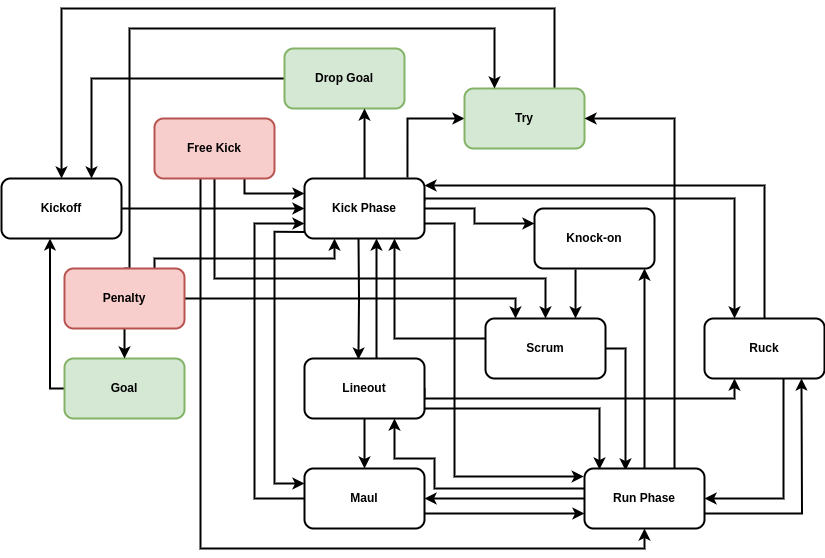
\includegraphics[width=14cm]{images/trywizard-event-graph.drawio.png}
\caption{Simplified event graph of a rugby union match.}
\label{fig:event-graph}
\end{figure}

In addition to occupying some state in the event graph, the state of a rugby match must also include a binary `possession' element which encodes which team has the ball at any moment. We should also include the 2-dimensional pitch location of the ball as an element of the match state in order to get a better sense of how likely some state transitions are, e.g., when playing on the edge of the pitch near the touchline it's clearly more likely that a {\sf Run Phase} is going to result in a {\sf Lineout} than if the state is currently in the centre of the pitch. To add even more detail; in the next section we will introduce states for each player.

Since a rugby match exists in continuous time, it is natural to choose a continuous-time event-based simulation model for our game engine. As we have discussed in previous chapters already, this means we will be characterising transition probabilities of the event graph in Fig.~\ref{fig:event-graph} by ratios of event rates in time. Recalling our notation in previous chapters, if we consider the current state vector of the match $X_{\sf t}$, we can start by assigning each transition ${\sf a}\rightarrow {\sf b}$ on the event graph an associated expected rate of occurance $\lambda_{{\sf a}\rightarrow {\sf b}}$ which is defined in units of continuous time, e.g., seconds. In addition to the transitions displayed on the graph, we can add a `possession change transition'; where the possession of the ball in play moves to the opposing team. This transition may occur while the match is also in any of the white-coloured states on the graph (apart from {\sf Knock-on} which determines a possession change immediately through a {\sf Scrum}) and let's assign this a state, parameter and timestep-dependent expected rate of occurance $\lambda_{\rm pos}(X_{\sf t}, z, {\sf t})$.

Based on our dicussion above, an appropriate encoding for the overall game state at timestep index ${\sf t}$ could be a state vector $X_{{\sf t}}$ whose elements are
%%
\begin{align}
X^0_{{\sf t}}&=\begin{cases} 0 & \text{Match State} = \text{{\sf Penalty}}\\ 1 & \text{Match State} = \text{{\sf Free Kick}} \\ \dots & \end{cases} \\
X^1_{{\sf t}}&=\begin{cases} 0 & \text{Possession} = \text{{\sf Home Team}}\\ 1 & \text{Possession} = \text{{\sf Away Team}} \end{cases} \,.
\end{align}
%%
But how does this overall game state connect to the event rates? The probabilistic answer is quite straightforward. If the probability of the match state being $X^0_{{\sf t}}={\sf a}$ at timestep ${\sf t}$ is written as $P^0_{{\sf t}}({\sf a})$, then the probability of $X^0_{{\sf t}+1}={\sf b}$ in the following timestep is
%%
\begin{align}
P^0_{{\sf t}+1}({\sf b}) = \frac{\frac{1}{\tau}P^0_{{\sf t}}({\sf b})+\sum_{\forall {\sf a}\neq {\sf b}}\lambda_{{\sf a}\rightarrow {\sf b}}{\cal T}_{{\sf a}\rightarrow {\sf b}}(X_{\sf t}, z, {\sf t})P^0_{{\sf t}}({\sf a})}{\big[ \frac{1}{\tau} + \sum_{\forall {\sf a}\neq {\sf b}}\lambda_{{\sf a}\rightarrow {\sf b}} {\cal T}_{{\sf a}\rightarrow {\sf b}}(X_{\sf t}, z, {\sf t})\big]} \label{eq:match-state-transition-probs}\,,
\end{align}
%%
where $\forall {\sf a} \neq {\sf b}$ in the summation indicates that all the available transitions from ${\sf a}$ to ${\sf b}$, where ${\sf a}\neq {\sf b}$, should be summed over and ${\cal T}_{{\sf a}\rightarrow {\sf b}}(X_{\sf t}, z, {\sf t})$ is a time, parameter and state-dependent transition probability that is determined by the playing tactics of each team as well as the general likelihoods of gameplay which are expected from a real rugby match. Note that in the expression above, we have also defined $\tau$ as a timescale short enough such that no transition is likely to occur during that interval. An equivalent to Eq.~(\ref{eq:match-state-transition-probs}) should also apply to the possession change transition rate, i.e., the probability that the {\sf Home Team} has possession $P^1_{{\sf t}}$ at time ${\sf t}$ evolves according to
%%
\begin{align}
P^1_{{\sf t}+1} = \frac{ \frac{1}{\tau}P^1_{{\sf t}} + \lambda_{\rm pos}(X_{\sf t}, z, {\sf t}) (1-P^1_{{\sf t}})}{\big[ \frac{1}{\tau} + \lambda_{\rm pos}(X_{\sf t}, z, {\sf t})\big]} \label{eq:possession-change-probs}\,.
\end{align}
%%

Before we move on to other details, it's quite important to recognise that because our process is defined in continuous time, the possession change rate may well vary continuously (this will be especially true when we talk about, e.g., player fatigue). Hence, Eq.~(\ref{eq:match-state-transition-probs}) is only an \emph{approximation} of the true underlying dynamics that we are trying to simulate --- and this approximation will only be accurate if $\tau$ is small. The reader may recall that we discussed this same issue from the point of view of simulating time-inhomogeneous Poisson processes with the rejection method when we were building the stochadex in an earlier chapter. 

While these match state transitions and possession changes are taking place, we also need to come up with a model for how the ball location $L_{{\sf t}}$ changes during the course of a game, and as a function of the current game state. Note that, because the ball location is a part of the overall game state, it will be included as information contained within some elements of $X_{{\sf t}}$ as well. To make this explicit, we can simply set $X^2_{{\sf t}}=L^{\rm lon}_{{\sf t}}$ and $X^3_{{\sf t}}=L^{\rm lat}_{{\sf t}}$ --- where $L^{\rm lon}_{{\sf t}}$ denotes the longitudinal component (lengthwise along the pitch) and $L^{\rm lat}_{{\sf t}}$ denotes the lateral component (widthwise across the pitch). If we associate every state on the event graph with a single change in spatial location of the ball on the pitch, we then need to construct a process which makes `jumps' in 2-dimensional space each time a state transition occurs. To keep things simple and intuitive, we will say that movements of the ball are only allowed to occur during either a {\sf Run Phase} or a {\sf Kick Phase}. 

In the case of a {\sf Run Phase}, let's choose the longitudinal component of the ball location $L^{\rm lon}_{{\sf t}}$ to be updated by the difference between samples drawn from two exponential distributions (one associated to each team). Hence, the probability density $P_{{\sf t}}(\ell )$ of $L^{\rm lon}_{{\sf t}}=\ell$ at timestep ${\sf t}$ evolves according to
%%
\begin{align}
P_{{\sf t}+1}(\ell ) = \int^\infty_0 {\rm d}\ell'\, {\sf ExponentialPDF}(\ell + \ell'; a_{\rm run}){\sf ExponentialPDF}(\ell'; d_{\rm run}) \label{eq:longitudinal-motion-rugby} \,,
\end{align}
%%
where $a_{\rm run}$ and $d_{\rm run}$ are the exponential distribution scale parameters for an attacking and defending player, respectively, and we have chosen positive values of $\ell$ to be aligned with the forward direction for the attacking team. We shall elaborate on where $a_{\rm run}$ and $d_{\rm run}$ come from when we discuss associating events for player abilities in due course. If we now consider lateral component of the ball location $L^{\rm lat}_{{\sf t}}$ during a {\sf Run Phase}; it makes sense that this wouldn't be affected much by either team within the scope of detail in this first version of our model. Hence, the probability density $P_{{\sf t}}(w)$ of $L^{\rm lat}_{{\sf t}}=w$ at timestep ${\sf t}$ can just be updated like so
%%
\begin{align}
P_{{\sf t}+1}(w) = {\sf NormalPDF}(w; L^{\rm lat}_{{\sf t}}, \sigma_{\rm run}^2) \label{eq:lateral-motion-rugby} \,,
\end{align}
%%
where $\sigma_{\rm run}$ is the typical jump in lateral motion (the standard deviation parameter of the normal distribution).

Turning our attention to the {\sf Kick Phase}; the longitudinal component is only realistically controlled by the attacking team. There's also an angular component to this motion which is associated to the direction that the kicker is orientating their kick. Therefore, the probability density of $P_{{\sf t}}(\ell )$ with $L^{\rm lon}_{{\sf t}}=\ell \cos \theta$ and $L^{\rm lat}_{{\sf t}}=\ell \sin \theta$ at timestep ${\sf t}$ will evolve according to
%%
\begin{align}
P_{{\sf t}+1}(\ell ) = {\sf ExponentialPDF}(\ell; a_{\rm kick}) \label{eq:longitudinal-motion-rugby-kicking} \,,
\end{align}
%%
where $a_{\rm kick}$ this time is the exponential scale parameter for the attacking team player who is kicking and $\theta$ is the angle they have chosen to kick at (where straight ahead is defined as $\theta = 0$). Similarly, the lateral component for a {\sf Kick Phase} is only going to be controlled by the accuracy of the kicker with the angle and longitudinal distance already applied. Therefore, the corresponding update to the probability density $P_{{\sf t}}(w)$ where $L^{\rm lon}_{{\sf t}}=w \sin \theta$ and $L^{\rm lat}_{{\sf t}}=w \cos \theta$ at timestep ${\sf t}$ will look like
%%
\begin{align}
P_{{\sf t}+1}(w) = {\sf NormalPDF}(w; L^{\rm lat}_{{\sf t}} + \ell \sin \theta, \sigma_{\rm kick}^2) \label{eq:lateral-motion-rugby-kicking} \,,
\end{align}
%%
with a standard deviation $\sigma_{\rm kick}$, and its interpretation now being the accuracy of the kicker.

\section{\sffamily Associating events to player states and abilities}

In the last section we introduced a continuous-time event-based simulation model for a rugby union match. In this section we are going to add more detail into this model by inventing how to associate specific player states and abilities to the event rates of the simulation. Before continuing, we want to reiterate that this model is entirely made up and, while we hope it illustrates some interesting mathematical modelling ideas in the context of rugby, there's no particular reason why a statistical inference with a reliable dataset should prefer our model to others which may exist.

In Fig.~\ref{fig:player-abilities} we began by separating playing positions on the rugby field into their usual descriptions and then associating each player type with a short list of simplified attributes. Our model is then to associate a player with an `possession attacking' and `possession defending' ability which corresponds to each of their attributes. For example, a Front Row Forward will have 8 abilities associated to them: 2 for each of their {\sf Scrum}, {\sf Lineout}, {\sf Ruck} and {\sf Maul} attributes.

\begin{figure}[h]
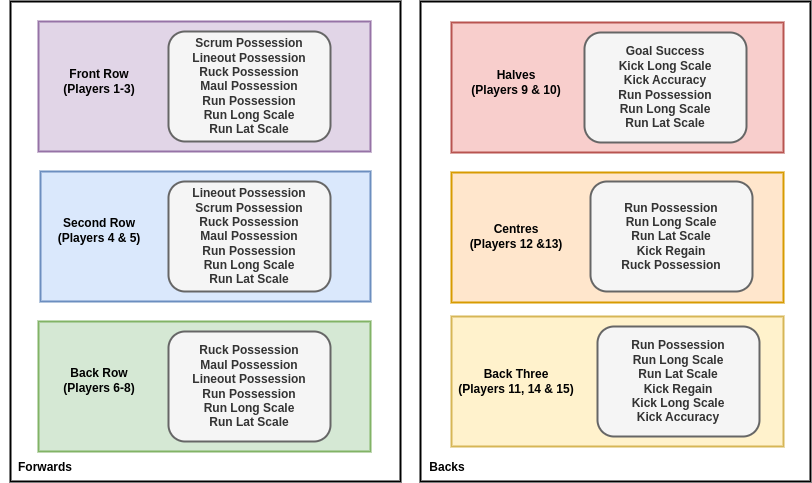
\includegraphics[width=15cm]{images/rugby-player-abilities.drawio.png}
\caption{Associated playing abilities for each position type.}
\label{fig:player-abilities}
\end{figure}

Let's now say that $z$ contains all of these parameters for all of the players on both sides, and also whether or not each player is actively playing or on the bench. With this information, and the knowledge of which team is in possession from $X^1_{\sf t}$, it should be simple to create a vector-valued function $a_{\rm pos}(X_{\sf t}, z)$ which returns all of the posession attacking attributes that are associated to match state $X^0_{\sf t}$ and an analogous one $d_{\rm pos}(X_{\sf t}, z)$ for the possession defending attributes. The dependencies of these functions on the ball possession state $X^1_{\sf t}$ comes from the fact that when, e.g., the {\sf Home Team} has possession of the ball it will be their possession attacking attributes that are returned by $a_{\rm pos}(X_{\sf t}, z)$ and the {\sf Away Team}'s possession defending attributes that are returned by $d_{\rm pos}(X_{\sf t}, z)$.

In order to model the effect of player fatigue over the course of a match, we can add some vectors of player fatigue values $f$ and times at which each player started playing $t_{\rm start}$ into the collection of parameters that are contained within $z$. These new parameters can then be used to define a formula for the decline of each attribute over the course of a match. Let's assign these declining values to be part of the overall match state like so
%%
\begin{align}
X^j_{\sf t} &= a^j_{\rm pos}(X_{\sf t}, z)e^{-f^j[t({\sf t})-t^j_{\rm start}]} \label{eq:att-player-fatigue} \\
X^k_{\sf t} &= d^k_{\rm pos}(X_{\sf t}, z)e^{-f^k[t({\sf t})-t^k_{\rm start}]} \label{eq:def-player-fatigue} \,,
\end{align}
%%
where the $j$ and $k$ each index the range of indices in the overall match state which correspond to the attacking and defending team player states, respectively.

So how does each player affect the events of a match? In our model, we would argue that players should be able to directly influence the possession change rate $\lambda_{\rm pos}(X_{\sf t}, z, {\sf t})$ through a balance of attacking and defensive attributes in the following relation
%%
\begin{align}
\lambda_{\rm pos}(X_{\sf t}, z, {\sf t}) &= \frac{\lambda^*_{\rm pos}\sum_{\forall j}X^j_{{\sf t}}}{\sum_{\forall j}X^j_{{\sf t}} + \sum_{\forall k}X^k_{{\sf t}}}\,,
\end{align}
%%
where $\lambda^*_{\rm pos}$ is the maximum rate that is physically possible and the $\forall j$ and $\forall k$ in the summations indicate summing over all attacking and defending player attributes, respectively. In addition to this possession change influence, players who have {\sf Run Phase} and {\sf Kick Phase} attributes may affect the gain in distance (and accuracy in the case of {\sf Kick Phase}) that each state translates to on the pitch. 

Let's first describe how we intend the {\sf Run Phase} to work. Every time the match state transitions into a {\sf Run Phase}, an individual player on the attacking side is chosen at random (uniformally across the team\footnote{This uniform sampling could be refined later to associate sampling probabilities with game state and player roles.}) to be the the nominal `attacker'. At the same time, an individual player on the defending side is chosen at random (again, uniformally across the team) to be the the nominal `defender'. Once these players have been chosen (and hence the $a_{\rm run}$ and $d_{\rm run}$ parameters have been determined), the longitudinal motion update we described in Eq.~(\ref{eq:longitudinal-motion-rugby}) can then be applied. Note that the $a_{\rm run}$ and $d_{\rm run}$ parameters should also receive a fatigue decrement depending on the time that each player has remained on the pitch, much like the exponential factors we applied in Eqs.~(\ref{eq:att-player-fatigue}) and~(\ref{eq:def-player-fatigue}).

Finally, we turn or attention to the mechanics of a {\sf Kick Phase}. For tactical kicking in the middle of play, this operates in a similar way as a {\sf Run Phase}; one of the players on the attacking side (the side in possession of the ball) is chosen at random (uniformally) and their $a_{\rm kick}$ and $\sigma_{\rm kick}$ attributes are used in Eqs.~(\ref{eq:longitudinal-motion-rugby-kicking}) and~(\ref{eq:lateral-motion-rugby-kicking}) to update the position of the ball. In the specific case of {\sf Goal} kicking from a {\sf Penalty}, the designated place kicker on each side also uses their same {\sf Kick Phase} attributes to determine the success/failure of the kick at the posts.

\section{\sffamily Deciding on managerial actions}

So how does managing a rugby match map to measured states and taking actions? To begin with, it makes sense to claim that the measurement of the total match state is perfect in this instance, and hence ${\cal S}_{{\sf t}}=X_{{\sf t}}$. We then have to figure out what sorts of managerial actions ${\cal A}_{{\sf t}}$ are parametric in nature (affecting $z$) and if any directly act on the state of the system itself (affecting $X_{\sf t}$). Let's jump straight to the answer to the second question --- we can't really think of any situation where the overall match state $X_{\sf t}$ itself is directly changed by a managerial action, so we will be using only parametric actions in this chapter.

Our model structure would suggest that the only way in which a manager can influence the state of a match is through modifying the parameters which are used by the $a_{\rm pos}(X_{\sf t},z)$, $d_{\rm pos}(X_{\sf t},z)$ or ${\cal T}_{{\sf a}\rightarrow {\sf b}}(X_{\sf t},z,{\sf t})$ functions. In the case of the possession attacking and defending attributes $a_{\rm pos}(X_{\sf t},z)$ and $d_{\rm pos}(X_{\sf t},z)$, a parametric action that the manager can perform would be to modify which players are actively playing through substitutions. To indicate that this underlying data may change, one can simply promote $z$ to its actionable, time-dependent counterpart $Z_{{\sf t}}$.

In addition to the changes that we have discussed above, we would argue that the parameters $a_{\sf run}$, $d_{\sf run}$, $a_{\rm kick}$ and $\sigma_{\rm kick}$ in Eqs.~(\ref{eq:longitudinal-motion-rugby}), (\ref{eq:longitudinal-motion-rugby-kicking}) and (\ref{eq:lateral-motion-rugby-kicking}) can also be determined by the manager to some extent through player selection/substitutions. 

\section{\sffamily Writing the game itself}

\begin{itemize}
\item{Show which stochadex/dexetera methods were called and how they were used to simulate the game.}
\item{Give a summary of how the dashboard backend works (diagram would help) and how this connects up to the streamlit frontend via protobuf messages.}
\end{itemize}

\part*{
\includegraphics*[width=14cm]{images/page-design-1.png}}

\chapter{\sffamily Influencing house prices}

{\bfseries\sffamily Concept.} The idea here is 

\part*{
\includegraphics*[width=14cm]{images/page-design-1.png}}

\part*{{\sffamily  Part 4. {\color{gray75} How do we then optimise the answer to Part 3 to achieve a specified control objective?}}
\includegraphics*[width=14cm]{images/page-design-1.png}}

\chapter{\sffamily Optimising actions for control objectives}

{\bfseries\sffamily Concept.} The idea here is 

\section{\sffamily States, actions and attributing rewards}

Up to this point, we have only considered actions which were either scheduled up front through some fixed process or through user interaction via a game interface. In order to start creating algorithms to act on the system state for us, we now need to develop a formalism which `closes the loop' by feeding information back from the stochastic process to another decision-making process. Note that in most cases, the state of real-world phenomena cannot be measured perfectly. So in order to enable any agent trained on simulated phenomena to potentially act in the real world, we will need to model this measurement process as part of the information retrieval step.

Let's now define the concept of a `measured state' ${\cal S}_{{\sf t}+1}$ of the system at timestep ${\sf t}+1$; this is a new vector that doesn't have to share the same length as $X_{{\sf t}+1}$. We can then say generally that this measured state is `observed' using the following measurement function
%%
\begin{align}
{\cal S}_{{\sf t}+1}^i &= M_{{\sf t}+1}^i(X',{\cal Z}_{{\sf t}+1},{\sf t}) \label{eq:generalised-state-measurement} \,,
\end{align}
%%
where we have also introduced a new vector ${\cal Z}_{{\sf t}+1}$ which we will use to store all of the relevant parameters to the agent\footnote{This vector is intended to include parameters for measurement, policy specification and ultimately the learning algorithm as well.} at timestep ${\sf t}+1$.

If we are now given the conditional probability that an action vector element ${\cal A}_{{\sf t}+1}=a$ is chosen given that state vector ${\cal S}_{{\sf t}+1}=s$ has been measured $\pi (a,s) = p(a\vert s)$, we can use this to draw new actions for the agent with a newly defined action-generating function
%%
\begin{align}
{\cal A}_{{\sf t}+1}^i &= \Pi_{{\sf t}+1}^i({\cal S}_{{\sf t}+1}, {\cal Z}_{{\sf t}+1}) \label{eq:action-generating-function} \,.
\end{align}
%%
From this point on we'll call $\pi (a,s)$ the `policy' adoped by the agent. A Markov Decision Process (MDP) defines an algorithm in which the agent uses a single state measurement vector and its given policy $\pi$ to draw actions ${\cal A}_{{\sf t}+1}$ at timestep ${{\sf t}+1}$. It then performs these actions in its environment, which we have previously formalised through defining the iteration $X_{{\sf t}+1} = {\cal F}_{{\sf t}+1}(X',Z_{\sf t},{\cal A}_{{\sf t}+1},{\sf t})$. 

In order to assess the quality of an agent's actions, we might later attribute a reward value ${\cal R}_{{\sf t}}$ for actions that were taken at timestep ${\sf t}$. Using a series of these rewards, a return value $R$ can also be computed using a future discount factor $\gamma$ like so 
%%
\begin{align}
R &= \sum_{{\sf t}=0}^\infty \gamma^{\sf t}{\cal R}_{\sf t} \,.
\end{align}
%%
A state-value function $V_\pi$ is defined as the expectation (under policy $\pi$) of return $R$, given state vector ${\cal S}_{\sf t}=s$, i.e.,
%%
\begin{align}
V_\pi (s) = {\rm E}_\pi (R\vert s) \,.
\end{align}
%%
Similarly, an action-value function $Q_\pi$ is defined as the expectation (again, under policy $\pi$) of return $R$, given state vector ${\cal S}_{\sf t}=s$ and action vector ${\cal A}_{\sf t}=a$, i.e.,
%%
\begin{align}
Q_\pi (s,a) = {\rm E}_\pi (R\vert s,a) \,.
\end{align}
%%

\part*{
\includegraphics*[width=14cm]{images/page-design-1.png}}

\chapter{\sffamily Resource allocation for epidemics}

{\bfseries\sffamily Concept.} The idea here is to limit the spread of some abstract epidemic through the correct time-dependent resource allocation.

\part*{
\includegraphics*[width=14cm]{images/page-design-1.png}}

\chapter{\sffamily Quantum system control}

{\bfseries\sffamily Concept.} The idea here is to follow stuff along these lines \href{https://arxiv.org/pdf/1210.7127.pdf}{here}. And also this sort of thing \href{https://en.wikipedia.org/wiki/Quantum_jump_method}{here} to simulate the Lindblad equation over an arbitrary network of entangled states.
 


%\appendix
%\chapter{First and only appendix}
\backmatter
\bibliographystyle{JHEP}
\bibliography{book}
\end{document}